\documentclass[10pt]{article}
\usepackage[polish]{babel}
\usepackage[utf8]{inputenc}
\usepackage[T1]{fontenc}
\usepackage{amsmath}
\usepackage{amsfonts}
\usepackage{amssymb}
\usepackage[version=4]{mhchem}
\usepackage{stmaryrd}
\usepackage{graphicx}
\usepackage[export]{adjustbox}
\graphicspath{ {./images/} }
\usepackage{mathrsfs}
\usepackage{fvextra, csquotes}

\title{EGZAMIN MATURALNY W ROKU SZKOLNYM 2014/2015 }

\author{}
\date{}


\newcommand\Varangle{\mathop{{<\!\!\!\!\!\text{\small)}}\:}\nolimits}

\begin{document}
\maketitle
FORMULA OD 2015\\
(„NOWA MATURA")

MATEMATYKA\\
POZIOM ROZSZERZONY

ZASADY OCENIANIA ROZWIĄZAŃ ZADAŃ\\
ARKUSZ MMA-R1

Uwaga: Akceptowane sq wszystkie odpowiedzi merytorycznie poprawne i spetniajace warunki zadania.

Zadanie 1. (0-1)

\begin{center}
\begin{tabular}{|c|l|c|}
\hline
\multicolumn{1}{|c|}{Wymagania ogólne} & \multicolumn{1}{c|}{Wymagania szczególowe} & \begin{tabular}{c}
Poprawna \\
odp. (1 p.) \\
\end{tabular} \\
\hline
\begin{tabular}{l}
II. Wykorzystanie \\
i interpretowanie \\
reprezentacji. \\
\end{tabular} & \begin{tabular}{l}
1. Liczby rzeczywiste. Zdający wykorzystuje \\
pojęcie wartości bezwzględnej i jej interpretację \\
geometryczną, zaznacza na osi liczbowej zbiory \\
opisane za pomocą równań i nierówności typu: \\
$|x-a|=b,|x-a|>b,|x-a|<b$ (R1.1). \\
\end{tabular} & D \\
\hline
\end{tabular}
\end{center}

\section*{Zadanie 2. (0-1)}
\begin{center}
\begin{tabular}{|l|l|l|}
\hline
\begin{tabular}{l}
II. Wykorzystanie \\
i interpretowanie \\
reprezentacji. \\
\end{tabular} & \begin{tabular}{l}
3. Równania i nierówności. Zdający rozwiązuje \\
równania i nierówności z wartością \\
bezwzględną (R3.9). \\
\end{tabular} & A \\
\hline
\end{tabular}
\end{center}

\section*{Zadanie 3. (0-1)}
II. Wykorzystanie i interpretowanie reprezentacji.\\
2. Wyrażenia algebraiczne. Zdający używa wzorów skróconego mnożenia na $(a \pm b)^{3}$ oraz $a^{3} \pm b^{3}$ (R2.1).

C\\
C\\
C

\section*{Zadanie 4. (0-1)}
\begin{center}
\begin{tabular}{|l|l|l|}
\hline
\begin{tabular}{l}
II. Wykorzystanie \\
i interpretowanie \\
reprezentacji. \\
\end{tabular} & \begin{tabular}{l}
6. Trygonometria. Zdający rozwiązuje równania \\
i nierówności trygonometryczne (R6.6). \\
\end{tabular} & A \\
\hline
\end{tabular}
\end{center}

Zadanie 5. (0-1)

\begin{center}
\begin{tabular}{|l|l|c|}
\hline
\begin{tabular}{l}
II. Wykorzystanie \\
i interpretowanie \\
reprezentacji. \\
\end{tabular} & \begin{tabular}{l}
8. Geometria na płaszczyźnie kartezjańskiej. \\
Zdający oblicza odległość punktu od prostej \\
(R8.4). \\
\end{tabular} & B \\
\hline
\end{tabular}
\end{center}

\section*{Zadanie 6. (0-2)}
Oblicz granice $\lim _{n \rightarrow \infty}\left(\frac{11 n^{3}+6 n+5}{6 n^{3}+1}-\frac{2 n^{2}+2 n+1}{5 n^{2}-4}\right)$. W poniższe kratki wpisz kolejno cyfrę jedności i pierwsze dwie cyfry po przecinku rozwinięcia dziesiętnego otrzymanego wyniku.\\
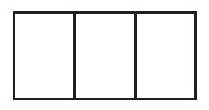
\includegraphics[max width=\textwidth, center]{2025_02_07_f5f4e8f37e6baab02e47g-03}\\
II. Wykorzystanie i interpretowanie reprezentacji.\\
5. Ciągi. Zdający oblicza granice ciągów, korzystając z granic ciągów typu $\frac{1}{n}, \frac{1}{n^{2}}$ oraz z twierdzeń o działaniach na granicach ciągów (R5.2).

Odpowiedź\\
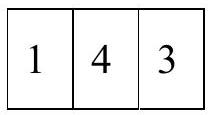
\includegraphics[max width=\textwidth, center]{2025_02_07_f5f4e8f37e6baab02e47g-03(1)}

\section*{Zadanie 7. (0-2)}
Liczby $(-1)$ i 3 są miejscami zerowymi funkcji kwadratowej $f$. Oblicz $\frac{f(6)}{f(12)}$.\\
II. Wykorzystanie i interpretowanie reprezentacji.\\
4. Funkcje. Zdający interpretuje współczynników występujących we wzorze funkcji kwadratowej w postaci kanonicznej, w postaci ogólnej i w postaci iloczynowej (4.10).

\section*{Rozwiązanie (I sposób)}
Zapisujemy trójmian kwadratowy w postaci iloczynowej

$$
f(x)=a(x+1)(x-3), \text { gdzie } a \neq 0
$$

Stąd zaś wynika, że

$$
\frac{f(6)}{f(12)}=\frac{a \cdot 7 \cdot 3}{a \cdot 13 \cdot 9}=\frac{7}{39} .
$$

\section*{Schemat oceniania}
\section*{Zdający otrzymuje}
gdy wykorzysta postać iloczynową funkcji kwadratowej i zapisze $f(6)=a \cdot 7 \cdot 3$ lub $f(12)=a \cdot 13 \cdot 9$ i na tym zakończy lub dalej popełni błędy.

Zdający otrzymuje. 2 p.\\
gdy obliczy wartość $\frac{f(6)}{f(12)}=\frac{7}{39}$.

\section*{Rozwiązanie (II sposób)}
Z wzorów Viète'a otrzymujemy $-\frac{b}{a}=2$ oraz $\frac{c}{a}=-3$. Stąd $b=-2 a$ oraz $c=-3 a$. Wzór funkcji $f$ możemy zapisać w postaci $f(x)=a x^{2}-2 a x-3 a$. Obliczamy wartości funkcji dla argumentów 6 i 12

$$
f(6)=36 a-12 a-3 a=21 a \text { oraz } f(12)=144 a-24 a-3 a=117 a .
$$

Zatem $\frac{f(6)}{f(12)}=\frac{21 a}{117 a}=\frac{7}{39}$.

\section*{Schemat oceniania}
$\qquad$\\
Zdający otrzymuje\\
gdy wykorzysta wzory Viète'a i zapisze $f(6)=36 a-12 a-3 a$ lub $f(12)=144 a-24 a-3 a$ i na tym zakończy lub dalej popełni błędy.\\
Zdający otrzymuje\\
gdy obliczy wartość $\frac{f(6)}{f(12)}=\frac{7}{39}$.

\section*{Zadanie 8. (0-3)}
Udowodnij, że dla każdej liczby rzeczywistej $x$ prawdziwa jest nierówność

$$
x^{4}-x^{2}-2 x+3>0 .
$$

\begin{center}
\begin{tabular}{|l|l|}
\hline
\begin{tabular}{r}
V. Rozumowanie \\
i argumentacja \\
\end{tabular} & \begin{tabular}{l}
2. Wyrażenia algebraiczne. Zdający dodaje, odejmuje, mnoży \\
i dzieli wyrażenia wymierne; rozszerza i (w łatwych \\
przykładach) skraca wyrażenia wymierne; używa wzory \\
skróconego mnożenia na $(a \pm b)^{2}, a^{2}-b^{2}$. (R2.6, 2.1). \\
\end{tabular} \\
\hline
\end{tabular}
\end{center}

\section*{Rozwiązanie (I sposób)}
Przekształćmy nierówność równoważnie w następujący sposób

$$
\begin{gathered}
x^{4}-2 x^{2}+1+x^{2}-2 x+1+1>0, \\
\left(x^{2}-1\right)^{2}+(x-1)^{2}+1>0 .
\end{gathered}
$$

Lewa strona tej nierówności jest sumą trzech składników, z których dwa pierwsze są nieujemne, a trzeci dodatni, więc suma ta jest dodatnia dla każdej liczby rzeczywistej $x$.

\section*{Schemat oceniania I sposobu rozwiązania}
Zdający otrzymuje 1 p.\\
gdy zapisze nierówność w postaci, z której lewą stronę łatwo można zapisać w postaci sumy składników nieujemnych: $x^{4}-2 x^{2}+1+x^{2}-2 x+1+1>0$.\\
Zdający otrzymuje 2 p.\\
gdy zapisze nierówność w postaci: $\left(x^{2}-1\right)^{2}+(x-1)^{2}+1>0$ i nie uzasadni prawdziwości tej nierówności.

\section*{Zdający otrzymuje}
gdy przeprowadzi pełne rozumowanie.

\section*{Rozwiązanie (II sposób)}
Przekształćmy nierówność równoważnie w następujący sposób

$$
\begin{gathered}
x^{4}-x^{2}-2 x+2+1>0, \\
x^{2}\left(x^{2}-1\right)-2(x-1)+1>0, \\
x^{2}(x-1)(x+1)-2(x-1)+1>0, \\
(x-1)\left(x^{2}(x+1)-2\right)+1>0, \\
(x-1)\left(x^{3}+x^{2}-2\right)+1>0, \\
(x-1)\left(x^{3}-x^{2}+2 x^{2}-2\right)+1>0, \\
(x-1)\left(x^{2}(x-1)+2\left(x^{2}-1\right)\right)+1>0 \\
(x-1)\left(x^{2}(x-1)+2(x-1)(x+1)\right)+1>0, \\
(x-1)^{2}\left(x^{2}+2(x+1)\right)+1>0, \\
(x-1)^{2}\left(x^{2}+2 x+1+1\right)+1>0, \\
(x-1)^{2}\left((x+1)^{2}+1\right)+1>0
\end{gathered}
$$

Ponieważ $(x-1)^{2} \geq 0$ oraz $(x+1)^{2}+1>0$ dla każdej liczby rzeczywistej $x$, więc iloczyn $(x-1)^{2}\left((x+1)^{2}+1\right)$ jest nieujemny. Stąd wynika, że lewa strona nierówności jest dodatnia dla każdej liczby rzeczywistej $x$.

\section*{Schemat oceniania II sposobu rozwiązania}
\section*{Zdający otrzymuje}
gdy zapisze nierówność w postaci: $x^{2}\left(x^{2}-1\right)-2(x-1)+1>0$.

\section*{Zdający otrzymuje}
gdy zapisze nierówność w postaci: $(x-1)^{2}\left(x^{2}+2 x+2\right)+1>0$ i nie uzasadni prawdziwości tej nierówności.

\section*{Zdający otrzymuje}
gdy przeprowadzi pełne rozumowanie.

\section*{Rozwiązanie (III sposób)}
Rozważmy wielomian $f(x)=x^{4}-x^{2}-2 x+3$.\\
Pochodna tego wielomianu jest równa $f^{\prime}(x)=4 x^{3}-2 x-2$ dla każdej liczby rzeczywistej $x$.\\
Ponieważ $f^{\prime}(1)=4-2-2=0$, więc wielomian $f^{\prime}$ jest podzielny przez dwumian $x-1$.\\
Wykorzystując schemat Hornera, otrzymujemy

\begin{center}
\begin{tabular}{|c|c|c|c|c|}
\hline
 & 4 & 0 & -2 & -2 \\
\hline
1 & 4 & 4 & 2 & 0 \\
\hline
\end{tabular}
\end{center}

Zatem $f^{\prime}(x)=(x-1)\left(4 x^{2}+4 x+2\right)$. Wyróżnik trójmianu kwadratowego $4 x^{2}+4 x+2$ jest równy $\Delta=4^{2}-4 \cdot 4 \cdot 2<0$, współczynnik przy $x^{2}$ jest dodatni, więc $4 x^{2}+4 x+2>0$ dla każdej liczby rzeczywistej $x$. Wynika stąd, że\\
$f^{\prime}(x)=0$ wtedy i tylko wtedy, gdy $x=1$,\\
$f^{\prime}(x)>0$ wtedy i tylko wtedy, gdy $x>1$,\\
$f^{\prime}(x)<0$ wtedy i tylko wtedy, gdy $x<1$.\\
To oznacza, że w punkcie $x=1$ wielomian $f$ osiąga minimum lokalne, które jest jednocześnie jego najmniejsza wartością, gdyż w przedziale $(-\infty, 1\rangle$ wielomian $f$ jest funkcją malejącą, a w przedziale $\langle 1,+\infty)$ rosnącą.\\
Ponieważ $f(1)=1^{4}-1^{2}-2 \cdot 1+3=1$, więc $f(x) \geq f(1)=1>0$, czyli $x^{4}-x^{2}-2 x+3>0$ dla każdej liczby rzeczywistej $x$. To kończy dowód.

\section*{Schemat oceniania III sposobu rozwiązania}
Zdający otrzymuje\\
gdy obliczy pochodną wielomianu $f(x)=x^{4}-x^{2}-2 x+3$, zapisze, że liczba 1 jest pierwiastkiem pochodnej: $f^{\prime}(x)=4 x^{3}-2 x-2, f^{\prime}(1)=4-2-2=0$.

Zdający otrzymuje 2 p.\\
gdy zapisze pochodną w postaci : $f^{\prime}(x)=(x-1)\left(4 x^{2}+4 x+2\right)$ i zbada znak pochodnej, ale nie przeprowadzi rozumowania do końca lub przeprowadzi je z błędem.\\
Zdający otrzymuje 3 p.\\
gdy przeprowadzi pełne rozumowanie.

\section*{Zadanie 9. (0-3)}
Dwusieczne czworokąta $A B C D$ wpisanego w okrąg przecinają się w czterech różnych punktach: $P, Q, R, S$ (zobacz rysunek).\\
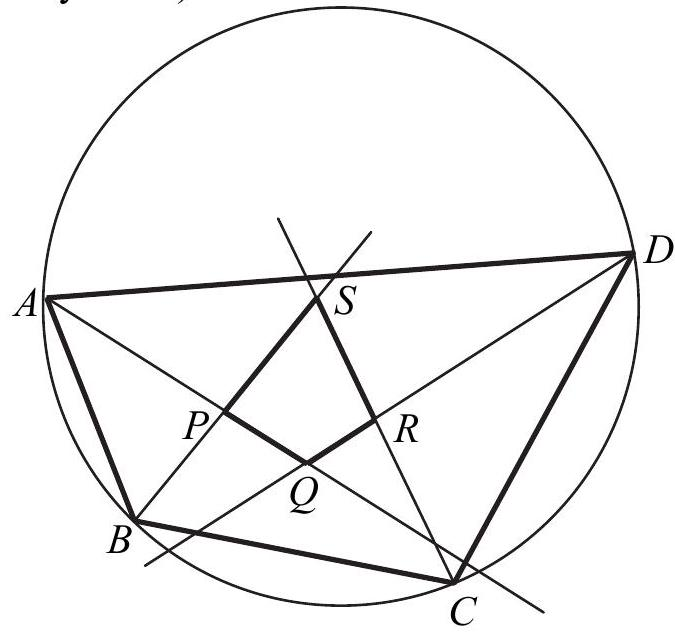
\includegraphics[max width=\textwidth, center]{2025_02_07_f5f4e8f37e6baab02e47g-07}

Wykaż, że na czworokącie $P Q R S$ można opisać okrąg.\\
V. Rozumowanie i argumentacja.\\
7. Planimetria. Zdający stosuje twierdzenia charakteryzujące czworokąty wpisane w okrąg i czworokąty opisane na okręgu (R7.1).

\section*{Rozwiązanie (I sposób)}
Oznaczmy $|\Varangle B A P|=|\Varangle P A D|=\alpha$ oraz $|\Varangle C B P|=|\Varangle A B P|=\beta$.\\
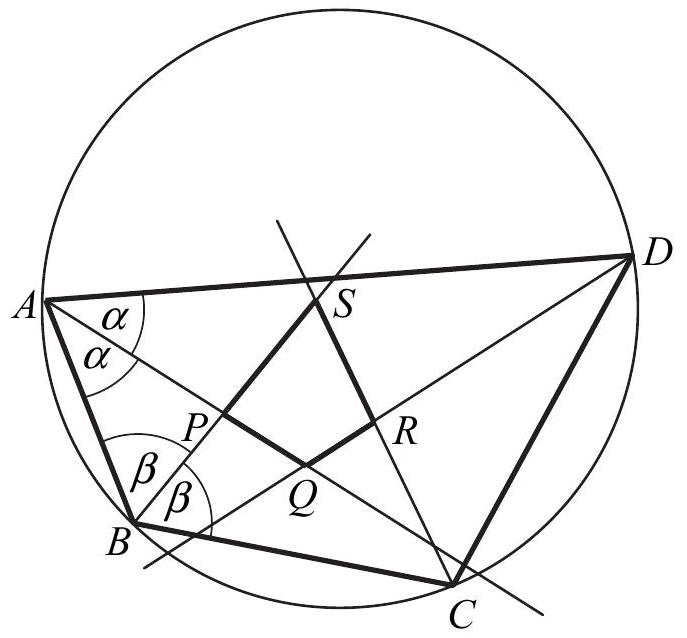
\includegraphics[max width=\textwidth, center]{2025_02_07_f5f4e8f37e6baab02e47g-07(1)}

Ponieważ czworokąt $A B C D$ jest wpisany w okrąg, więc

$$
|\Varangle B C R|=\frac{180^{\circ}-2 \alpha}{2}=90^{\circ}-\alpha \text { oraz }|\Varangle A D R|=\frac{180^{\circ}-2 \beta}{2}=90^{\circ}-\beta .
$$

Zauważmy, że

$$
|\Varangle A Q D|=180^{\circ}-(|\Varangle D A Q|+|\Varangle A D Q|)=180^{\circ}-\left(\alpha+\left(90^{\circ}-\beta\right)\right)=90^{\circ}-\alpha+\beta
$$

oraz

$$
|\Varangle B S C|=180^{\circ}-(|\Varangle B C R|+|\Varangle C B P|)=180^{\circ}-\left(\left(90^{\circ}-\alpha\right)+\beta\right)=90^{\circ}+\alpha-\beta
$$

Zatem

$$
|\Varangle P Q R|+|\Varangle P S R|=\left(90^{\circ}-\alpha+\beta\right)+\left(90^{\circ}+\alpha-\beta\right)=180^{\circ} .
$$

Suma wszystkich kątów czworokąta jest równa $360^{\circ}$, więc suma pozostałych dwóch kątów czworokąta $P Q R S$ także jest równa $180^{\circ}$. To oznacza, że na czworokącie $P Q R S$ można opisać okrąg, co kończy dowód.

Schemat oceniania I sposobu rozwiązania\\
Zdający otrzymuje\\
gdy przyjmie oznaczenia dwóch sąsiednich kątów wewnętrznych czworokąta $A B C D$ (lub oznaczy połowy tych kątów) np.: $|\Varangle B A P|=|\Varangle P A D|=\alpha,|\Varangle C B P|=|\Varangle A B P|=\beta$ oraz zapisze dwa pozostałe kąty wewnętrzne tego czworokąta (lub ich połowy) w zależności od $\alpha$ i $\beta$ : $|\Varangle B C R|=|\Varangle D C R|=90^{\circ}-\alpha,|\Varangle C D R|=|\Varangle A D R|=90^{\circ}-\beta$.\\
Zdający otrzymuje\\
gdy wyznaczy dwa przeciwległe kąty czworokąta $P Q R S$ w zależności od $\alpha$ i $\beta$ : $|\Varangle A Q D|=90^{\circ}-\alpha+\beta,|\Varangle B S C|=90^{\circ}+\alpha-\beta$.\\
Zdający otrzymuje 3 p.\\
gdy wykaże, że suma dwóch przeciwległych kątów wewnętrznych czworokąta $P Q R S$ jest równa $180^{\circ}$.

\section*{Rozwiązanie (II sposób)}
Oznaczmy $|\Varangle B A P|=|\Varangle P A D|=\alpha$ oraz $|\Varangle C B P|=|\Varangle A B P|=\beta$.\\
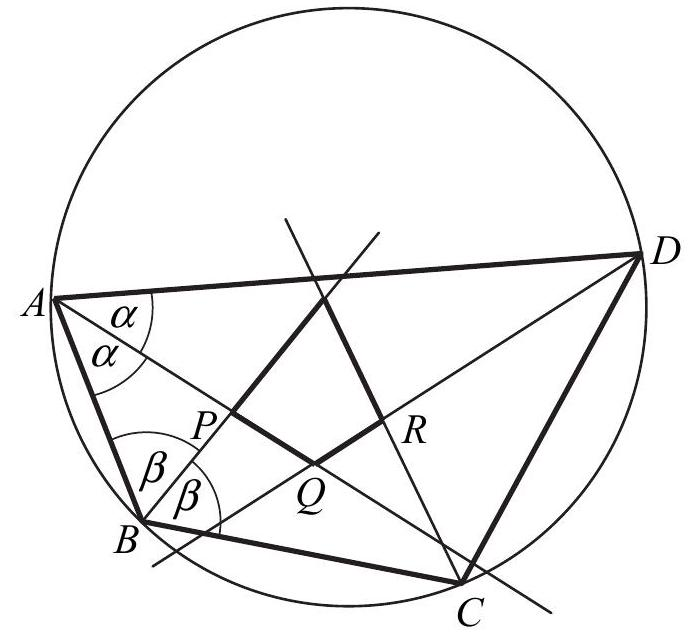
\includegraphics[max width=\textwidth, center]{2025_02_07_f5f4e8f37e6baab02e47g-08}

Ponieważ czworokąt $A B C D$ jest wpisany w okrąg, więc

$$
|\Varangle B C R|=|\Varangle D C R|=\frac{180^{\circ}-2 \alpha}{2}=90^{\circ}-\alpha \text { oraz }|\Varangle C D R|=|\Varangle A D R|=\frac{180^{\circ}-2 \beta}{2}=90^{\circ}-\beta .
$$

Zauważmy, że

$$
|\Varangle S P Q|=|\Varangle A P B|=180^{\circ}-(|\Varangle A B P|+|\Varangle B A P|)=180^{\circ}-(\alpha+\beta)
$$

oraz

$$
|\Varangle S R Q|=|\Varangle C R D|=180^{\circ}-(|\Varangle D C R|+|\Varangle C D R|)=180^{\circ}-\left(\left(90^{\circ}-\alpha\right)+\left(90^{\circ}-\beta\right)\right)=\alpha+\beta .
$$

Zatem

$$
|\Varangle S P Q|+|\Varangle S R Q|=180^{\circ}-(\alpha+\beta)+\alpha+\beta=180^{\circ} .
$$

Suma wszystkich kątów czworokąta jest równa $360^{\circ}$, więc suma pozostałych dwóch kątów czworokąta $P Q R S$ także jest równa $180^{\circ}$. To oznacza, że na czworokącie $P Q R S$ można opisać okrąg, co kończy dowód.

\section*{Schemat oceniania II sposobu rozwiązania}
Zdający otrzymuje 1 p. gdy przyjmie oznaczenia dwóch sąsiednich kątów wewnętrznych czworokąta $A B C D$ (lub oznaczy połowy tych kątów) np.: $|\Varangle B A P|=|\Varangle P A D|=\alpha,|\Varangle C B P|=|\Varangle A B P|=\beta$ oraz zapisze dwa pozostałe kąty wewnętrzne tego czworokąta (lub ich połowy) w zależności od $\alpha$ i $\beta$ : $|\Varangle B C R|=|\Varangle D C R|=90^{\circ}-\alpha,|\Varangle C D R|=|\Varangle A D R|=90^{\circ}-\beta$.

\section*{Zdający otrzymuje}
gdy wyznaczy dwa przeciwległe kąty czworokąta $P Q R S$ w zależności od $\alpha$ i $\beta$ : $|\Varangle S P Q|=180^{\circ}-(\alpha+\beta),|\Varangle S R Q|=\alpha+\beta$.

\section*{Zdający otrzymuje}
 3 p.gdy wykaże, że suma dwóch przeciwległych kątów wewnętrznych czworokąta $P Q R S$ jest równa $180^{\circ}$.

\section*{Rozwiązanie (III sposób)}
Oznaczmy: $|\Varangle B A P|=|\Varangle D A P|=\alpha,|\Varangle C B P|=|\Varangle A B P|=\beta,|\Varangle D C R|=|\Varangle B C R|=\gamma$, $|\Varangle A D R|=|\Varangle C D R|=\delta$.\\
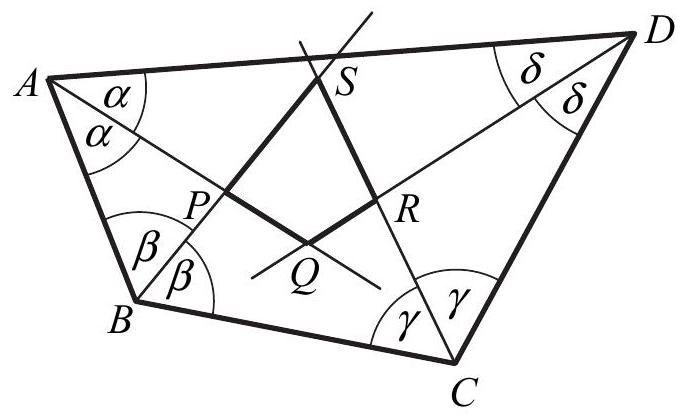
\includegraphics[max width=\textwidth, center]{2025_02_07_f5f4e8f37e6baab02e47g-09}

Suma kątów czworokąta $A B C D$ jest równa

$$
2 \alpha+2 \beta+2 \gamma+2 \delta=360^{\circ}
$$

Stąd


\begin{equation*}
\alpha+\beta+\gamma+\delta=180^{\circ} \tag{1}
\end{equation*}


Z bilansu kątów w trójkątach $A D Q$ i $B C S$ otrzymujemy

$$
|\Varangle A Q D|=180^{\circ}-(\alpha+\delta) \text { oraz }|\Varangle B S C|=180^{\circ}-(\beta+\gamma) .
$$

Suma przeciwległych kątów $P Q R$ i $P S R$ czworokąta $P Q R S$ jest więc równa

$$
|\Varangle P Q R|+|\Varangle P S R|=180^{\circ}-(\alpha+\delta)+180^{\circ}-(\beta+\gamma)=360^{\circ}-(\alpha+\beta+\gamma+\delta) .
$$

Stąd i z (1) otrzymujemy

$$
|\Varangle P Q R|+|\Varangle P S R|=360^{\circ}-180^{\circ}=180^{\circ} .
$$

To oznacza, że suma pozostałych dwóch kątów czworokąta $P Q R S$ także jest równa $180^{\circ}$. Zatem na czworokącie PQRS można opisać okrạg. To kończy dowód.

\section*{Rozwiązanie (IV sposób)}
Oznaczmy: $|\Varangle B A P|=|\Varangle D A P|=\alpha,|\Varangle C B P|=|\Varangle A B P|=\beta,|\Varangle D C R|=|\Varangle B C R|=\gamma$, $|\Varangle A D R|=|\Varangle C D R|=\delta$.\\
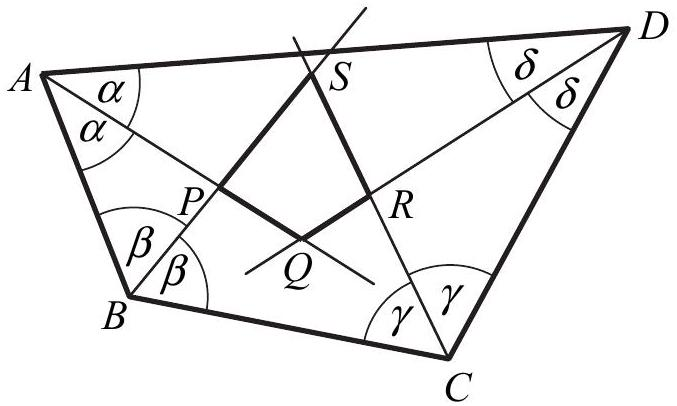
\includegraphics[max width=\textwidth, center]{2025_02_07_f5f4e8f37e6baab02e47g-10}

Suma kątów czworokąta $A B C D$ jest równa

$$
2 \alpha+2 \beta+2 \gamma+2 \delta=360^{\circ} .
$$

Stąd


\begin{equation*}
\alpha+\beta+\gamma+\delta=180^{\circ} . \tag{1}
\end{equation*}


Z bilansu kątów w trójkątach $A B P$ i $C D R$ otrzymujemy

$$
|\Varangle B P A|=180^{\circ}-(\alpha+\beta) \text { oraz }|\Varangle C R D|=180^{\circ}-(\gamma+\delta) .
$$

Kąty $B P A$ i $S P Q$ są wierzchołkowe, podobnie jak kąty $C R D$ i $S R Q$. Zatem

$$
|\Varangle S P Q|=180^{\circ}-(\alpha+\beta) \text { oraz }|\Varangle S R Q|=180^{\circ}-(\gamma+\delta) .
$$

Suma przeciwległych kątów $S P Q$ i $S R Q$ czworokąta $P Q R S$ jest więc równa

$$
|\Varangle S P Q|+|\Varangle S R Q|=180^{\circ}-(\alpha+\beta)+180^{\circ}-(\gamma+\delta)=360^{\circ}-(\alpha+\beta+\gamma+\delta) .
$$

Stąd i z (1) otrzymujemy

$$
|\Varangle S P Q|+|\Varangle S R Q|=360^{\circ}-180^{\circ}=180^{\circ} .
$$

To oznacza, że suma pozostałych dwóch kątów czworokąta PQRS także jest równa $180^{\circ}$. Zatem na czworokącie PQRS można opisać okrąg. To kończy dowód.

\section*{Schemat oceniania III i IV sposobu rozwiązania Zdający otrzymuje}
i zapisze:

\begin{itemize}
  \item że ich suma jest równa $360^{\circ}: 2 \alpha+2 \beta+2 \gamma+2 \delta=360^{\circ}$\\
albo
  \item wyznaczy dwa przeciwległe kąty $P Q R$ i $P S R$ czworokąta $P Q R S$ w zależności od
\end{itemize}

$$
\alpha, \beta, \gamma \text { i } \delta:|\Varangle P Q R|=180^{\circ}-(\alpha+\delta),|\Varangle P S R|=180^{\circ}-(\beta+\gamma)
$$

albo

\begin{itemize}
  \item wyznaczy dwa przeciwległe kąty $S P Q$ i $S R Q$ czworokąta $P Q R S$ w zależności od $\alpha, \beta, \gamma$ i $\delta:|\Varangle S P Q|=180^{\circ}-(\alpha+\beta),|\Varangle S R Q|=180^{\circ}-(\gamma+\delta)$.
\end{itemize}

\section*{Zdający otrzymuje}
gdy zapisze, że $2 \alpha+2 \beta+2 \gamma+2 \delta=360^{\circ}$ oraz

\begin{itemize}
  \item wyznaczy dwa przeciwległe kąty $P Q R$ i $P S R$ czworokąta $P Q R S$ w zależności od $\alpha, \beta, \gamma$ i $\delta:|\Varangle P Q R|=180^{\circ}-(\alpha+\delta),|\Varangle P S R|=180^{\circ}-(\beta+\gamma)$\\
albo
  \item wyznaczy dwa przeciwległe kąty $S P Q$ i $S R Q$ czworokąta $P Q R S$ w zależności od $\alpha, \beta, \gamma$ i $\delta:|\Varangle S P Q|=180^{\circ}-(\alpha+\beta),|\Varangle S R Q|=180^{\circ}-(\gamma+\delta)$.
\end{itemize}

\section*{Zdający otrzymuje.}
gdy wykaże, że suma dwóch przeciwległych kątów wewnętrznych czworokąta $P Q R S$ jest równa $180^{\circ}$.

Zadanie 10. (0-4)\\
Długości boków czworokąta $A B C D$ są równe: $|A B|=2,|B C|=3,|C D|=4,|D A|=5$. Na czworokącie $A B C D$ opisano okrąg. Oblicz długość przekątnej $A C$ tego czworokąta.

\section*{IV. Użycie i tworzenie strategii.}
\begin{enumerate}
  \setcounter{enumi}{6}
  \item Planimetria. Zdający stosuje twierdzenia charakteryzujące czworokąty wpisane w okrąg i czworokąty opisane na okręgu; znajduje związki miarowe w figurach płaskich z zastosowaniem twierdzenia sinusów i twierdzenia cosinusów (R7.1, R7.5).
\end{enumerate}

\section*{Rozwiązanie (I sposób)}
Przyjmijmy oznaczenia $a=|A B|=2, b=|B C|=3, c=|C D|=4, d=|D A|=5, x=|A C|$, $\alpha=|\Varangle A B C|$ jak na rysunku.\\
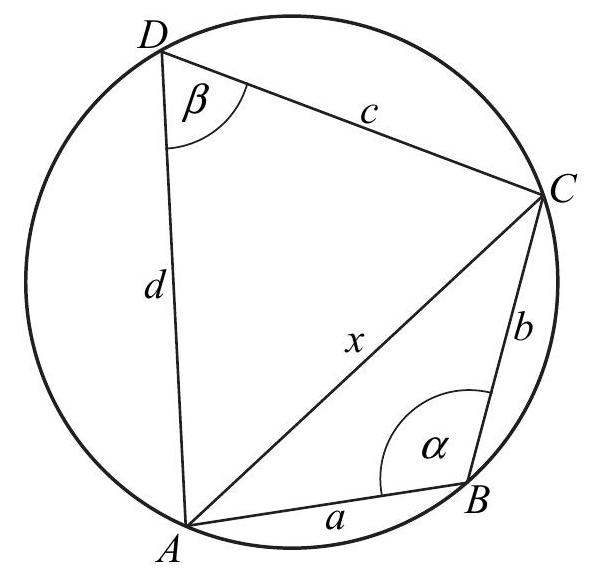
\includegraphics[max width=\textwidth, center]{2025_02_07_f5f4e8f37e6baab02e47g-11}

Ponieważ na czworokącie $A B C D$ jest opisany okrąg, więc $|\Varangle C D A|=180^{\circ}-\alpha$.\\
Z twierdzenia cosinusów zastosowanego do trójkąta $A B C$ otrzymujemy:

$$
|A C|^{2}=|A B|^{2}+|B C|^{2}-2 \cdot|A B| \cdot|B C| \cdot \cos \alpha
$$


\begin{equation*}
|A C|^{2}=2^{2}+3^{2}-2 \cdot 2 \cdot 3 \cdot \cos \alpha \tag{1}
\end{equation*}


Teraz ponownie zastosujemy twierdzenie cosinusów, tym razem do trójkąta $A C D$ :

$$
|A C|^{2}=|C D|^{2}+|D A|^{2}-2 \cdot|C D| \cdot|D A| \cdot \cos \left(180^{\circ}-\alpha\right)
$$


\begin{equation*}
|A C|^{2}=4^{2}+5^{2}+2 \cdot 4 \cdot 5 \cdot \cos \alpha . \tag{2}
\end{equation*}


Porównujemy prawe strony równań (1) i (2):

$$
\begin{aligned}
2^{2}+3^{2}-2 \cdot 2 \cdot 3 \cdot \cos \alpha & =4^{2}+5^{2}+2 \cdot 4 \cdot 5 \cdot \cos \alpha \\
13-12 \cdot \cos \alpha & =41+40 \cdot \cos \alpha
\end{aligned}
$$

$$
\cos \alpha=-\frac{28}{52}=-\frac{7}{13} .
$$

Podstawiamy otrzymaną wartość do równania (1) i otrzymujemy:

$$
|A C|^{2}=13-12 \cdot\left(-\frac{7}{13}\right)=13+\frac{84}{13}=\frac{169+84}{13}=\frac{253}{13} .
$$

Stąd wynika, że długość przekątnej $A C$ jest równa:

$$
|A C|=\sqrt{\frac{253}{13}} .
$$

\section*{Uwaga}
Układ równań (1) i (2) możemy rozwiązać rugując $\cos \alpha$. Wtedy mnożymy obie strony równania (1) przez 10, a obie strony równania (2) przez 3 i mamy

$$
10 x^{2}=10 \cdot 4+10 \cdot 9-120 \cdot \cos \alpha \text { oraz } 3 x^{2}=3 \cdot 16+3 \cdot 25+120 \cdot \cos \alpha \text {. }
$$

Dodając stronami otrzymane równania mamy

$$
13 x^{2}=253
$$

Stąd

$$
x=|A C|=\sqrt{\frac{253}{13}} .
$$

\section*{Schemat oceniania I sposobu rozwiazania}
Rozwiązanie, w którym postęp jest niewielki, ale konieczny na drodze do pełnego rozwiązania\\
Zdający zapisze równanie wynikające z twierdzenia cosinusów zastosowanego do trójkąta $A B C$ albo do trójkąta $C D A$ :

$$
x^{2}=2^{2}+3^{2}-2 \cdot 2 \cdot 3 \cdot \cos \alpha \text { albo } x^{2}=4^{2}+5^{2}-2 \cdot 4 \cdot 5 \cdot \cos \beta
$$

i na tym zakończy lub dalej popełni błędy.\\
Rozwiązanie, w którym jest istotny postęp 2 p.\\
Zdający zapisze

\begin{itemize}
  \item równanie $z$ jedną niewiadomą, np.:
\end{itemize}

$$
2^{2}+3^{2}-2 \cdot 2 \cdot 3 \cdot \cos \alpha=4^{2}+5^{2}-2 \cdot 4 \cdot 5 \cdot \cos \left(180^{\circ}-\alpha\right)
$$

albo

\begin{itemize}
  \item układ równań w postaci:
\end{itemize}

$$
10 x^{2}=10 \cdot 4+10 \cdot 9-120 \cdot \cos \alpha \text { i } 3 x^{2}=3 \cdot 16+3 \cdot 25+120 \cdot \cos \alpha \text {. }
$$

i na tym zakończy lub dalej popełni błędy.

\section*{Pokonanie zasadniczych trudności zadania 3 p. Zdający}
\begin{itemize}
  \item obliczy cosinus kąta $A B C: \cos a=-\frac{7}{13}$\\
albo
  \item zapisze równanie z niewiadomą $x$, np.: $13 x^{2}=253$.
\end{itemize}

Rozwiązanie pelne 4 p.\\
Zdający obliczy długość przekątnej $A C$ : $|A C|=\sqrt{\frac{253}{13}}$.

\section*{Rozwiązanie (II sposób)}
Przyjmijmy oznaczenia $x=|A C| y=|B D|$ jak na rysunku i niech $R$ oznacza promień okręgu opisanego na czworokącie $A B C D$.\\
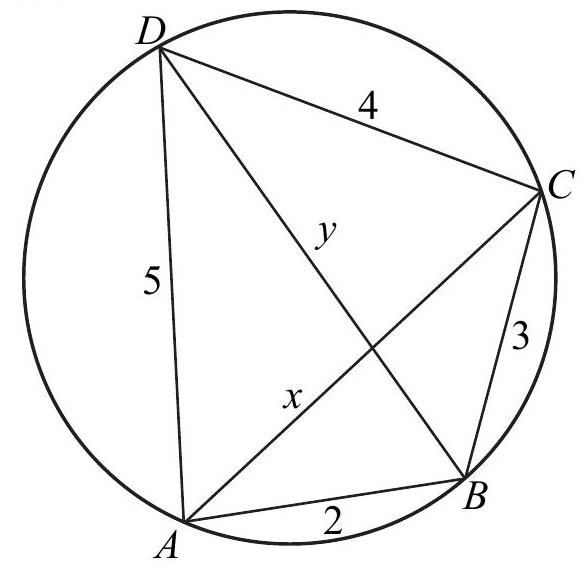
\includegraphics[max width=\textwidth, center]{2025_02_07_f5f4e8f37e6baab02e47g-13}

Z twierdzenia Ptolemeusza otrzymujemy równanie

$$
\begin{gathered}
x y=2 \cdot 4+5 \cdot 3 \\
x y=23 .
\end{gathered}
$$

Okrąg opisany na czworokącie $A B C D$ jest jednocześnie okręgiem opisanym na każdym z trójkątów $A B C, B C D, C D A$ i $A B D$. Pole czworokąta $A B C D$ możemy zapisać na dwa sposoby

$$
P_{A B C D}=P_{A B C}+P_{C D A}=P_{B C D}+P_{A B D} .
$$

Stąd i ze wzoru na pole trójkąta $P=\frac{a b c}{4 R}$ otrzymujemy równanie

$$
\begin{aligned}
\frac{2 \cdot 3 \cdot x}{4 R}+\frac{4 \cdot 5 \cdot x}{4 R} & =\frac{2 \cdot 5 \cdot y}{4 R}+\frac{3 \cdot 4 \cdot y}{4 R} \\
26 x & =22 y \\
y & =\frac{13}{11} x
\end{aligned}
$$

Stąd i z równości $x y=23$ otrzymujemy

$$
\begin{gathered}
x \cdot \frac{13}{11} x=23, \\
x^{2}=\frac{23 \cdot 11}{13} \\
x=\sqrt{\frac{253}{13}}
\end{gathered}
$$

\section*{Schemat oceniania II sposobu rozwiązania}
Rozwiązanie, w którym postęp jest niewielki, ale konieczny na drodze do pełnego rozwiązania 1 p.\\
Zdający zapisze

\begin{itemize}
  \item równanie wynikające z twierdzenia Ptolemeusza: $x y=2 \cdot 4+5 \cdot 3$\\
albo
  \item pole czworokąta $A B C D$ na dwa sposoby i zapisze $P_{A B C}+P_{C D A}=P_{B C D}+P_{A B D}$ lub $\frac{2 \cdot 3 \cdot x}{4 R}+\frac{4 \cdot 5 \cdot x}{4 R}=\frac{2 \cdot 5 \cdot y}{4 R}+\frac{3 \cdot 4 \cdot y}{4 R}$.\\
i na tym zakończy lub dalej popełni błędy.\\
Rozwiązanie, w którym jest istotny postęp ..... 2 p.Zdający zapisze układ równań z niewiadomymi $x$ i $y$ :$x y=2 \cdot 4+5 \cdot 3$ oraz $2 \cdot 3 \cdot x+4 \cdot 5 \cdot x=2 \cdot 5 \cdot y+3 \cdot 4 \cdot y$.i na tym zakończy lub dalej popełni błędy.\\
Pokonanie zasadniczych trudności zadania3 p.Zdający zapisze równanie z jedną niewiadomą, np.: $x \cdot \frac{13}{11} x=23$ lub $\frac{11}{13} y \cdot y=23$.Rozwiązanie petne4 p.Zdający obliczy długość przekątnej $A C: x=|A C|=\sqrt{\frac{253}{13}}$.
\end{itemize}

\section*{Zadanie 11. (0-4)}
W pierwszej urnie umieszczono 3 kule białe i 5 kul czarnych, a w drugiej urnie 7 kul białych i 2 kule czarne. Losujemy jedną kulę z pierwszej urny, przekładamy ją do urny drugiej i dodatkowo dokładamy do urny drugiej jeszcze dwie kule tego samego koloru, co wylosowana kula. Następnie losujemy dwie kule z urny drugiej. Oblicz prawdopodobieństwo zdarzenia polegającego na tym, że obie kule wylosowane z drugiej urny będą białe.

\begin{center}
\begin{tabular}{|c|l|}
\hline
\begin{tabular}{c}
IV. Użycie i tworzenie \\
strategii. \\
\end{tabular} & \begin{tabular}{l}
10. Elementy statystyki opisowej. Teoria prawdopodobieństwa \\
i kombinatoryka. Zdający korzysta z twierdzenia \\
o prawdopodobieństwie całkowitym (R10.3). \\
\end{tabular} \\
\hline
\end{tabular}
\end{center}

\section*{Rozwiązanie (I sposób)}
Przyjmijmy następujące oznaczenia zdarzeń:\\
$A$ - zdarzenie polegające na tym, że z drugiej urny wylosujemy dwie kule białe,\\
$B_{1}$ - zdarzenie polegające na tym, że z pierwszej urny wylosujemy kulę białą.\\
$B_{2}$ - zdarzenie polegające na tym, że z pierwszej urny wylosujemy kulę czarną.\\
Wówczas $B_{1} \cap B_{2}=\varnothing$ oraz $B_{1} \cup B_{2}=\Omega$. Następnie

$$
P\left(B_{1}\right)=\frac{3}{8}>0 \text { oraz } P\left(B_{2}\right)=\frac{5}{8}>0 .
$$

Zatem spełnione są założenia twierdzenia o prawdopodobieństwie całkowitym. Obliczamy teraz prawdopodobieństwa warunkowe:

$$
P\left(A \mid B_{1}\right)=\frac{\binom{10}{2}}{\binom{12}{2}}=\frac{15}{22} \text { oraz } P\left(A \mid B_{2}\right)=\frac{\binom{7}{2}}{\binom{12}{2}}=\frac{7}{22} .
$$

Z twierdzenia o prawdopodobieństwie całkowitym otrzymujemy\\
$P(A)=P\left(A \mid B_{1}\right) \cdot P\left(B_{1}\right)+P\left(A \mid B_{2}\right) \cdot P\left(B_{2}\right)=\frac{15}{22} \cdot \frac{3}{8}+\frac{7}{22} \cdot \frac{5}{8}=\frac{45+35}{8 \cdot 22}=\frac{80}{8 \cdot 22}=\frac{5}{11}$.

\section*{Schemat oceniania I sposobu rozwiązania}
Rozwiązanie, w którym postęp jest niewielki, ale konieczny na drodze do pełnego rozwiązania\\
Zdający opisze zdarzenia $A, B_{1}$ i $B_{2}$.

\section*{Rozwiązanie, w którym jest istotny postęp 2 p. \\
 Zdający}
\begin{itemize}
  \item obliczy prawdopodobieństwa $P\left(B_{1}\right)=\frac{3}{8}$ oraz $P\left(B_{2}\right)=\frac{5}{8}$\\
albo
  \item obliczy prawdopodobieństwa $P\left(A \mid B_{1}\right)=\frac{15}{22}, P\left(A \mid B_{2}\right)=\frac{7}{22}$\\
albo
  \item obliczy prawdopodobieństwa $P\left(B_{1}\right)=\frac{3}{8}$ oraz $P\left(A \mid B_{1}\right)=\frac{15}{22}$\\
albo
  \item obliczy prawdopodobieństwa $P\left(B_{2}\right)=\frac{5}{8}$ oraz $P\left(A \mid B_{2}\right)=\frac{7}{22}$.
\end{itemize}

\section*{Pokonanie zasadniczych trudności zadania.}
Zdający obliczy prawdopodobieństwa: $P\left(B_{1}\right)=\frac{3}{8}, P\left(B_{2}\right)=\frac{5}{8}, P\left(A \mid B_{1}\right)=\frac{15}{22}$,\\
$P\left(A \mid B_{2}\right)=\frac{7}{22}$.\\
Rozwiązanie pelne 4 p.\\
Zdający obliczy prawdopodobieństwo: $P(A)=\frac{5}{11}$.

\section*{Rozwiązanie (II sposób)}
Przyjmijmy, że $A$ to zdarzenie polegające na tym, że z drugiej urny wylosujemy dwie kule białe. Rysujemy drzewo z istotnymi gałęziami\\
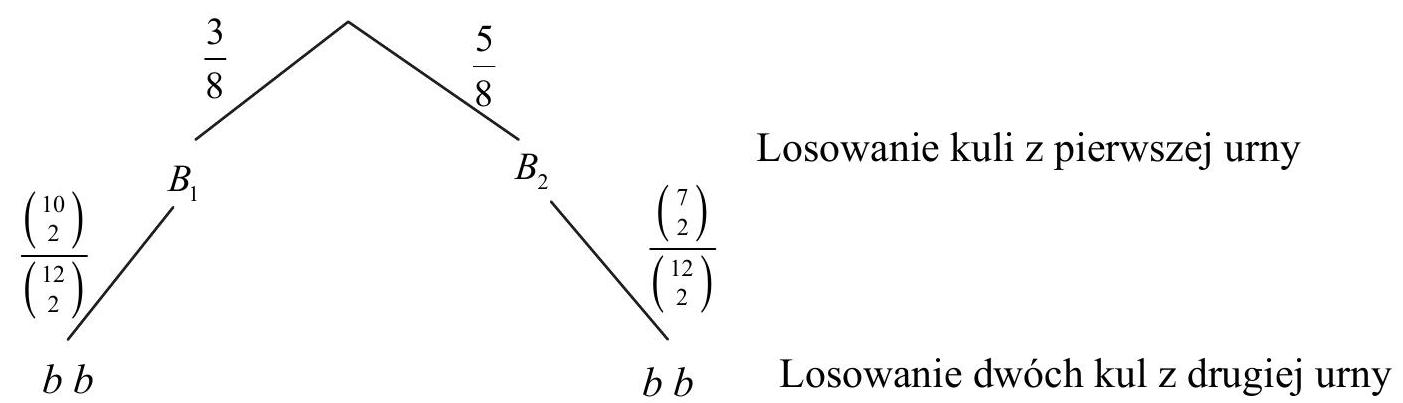
\includegraphics[max width=\textwidth, center]{2025_02_07_f5f4e8f37e6baab02e47g-16}\\
lub\\
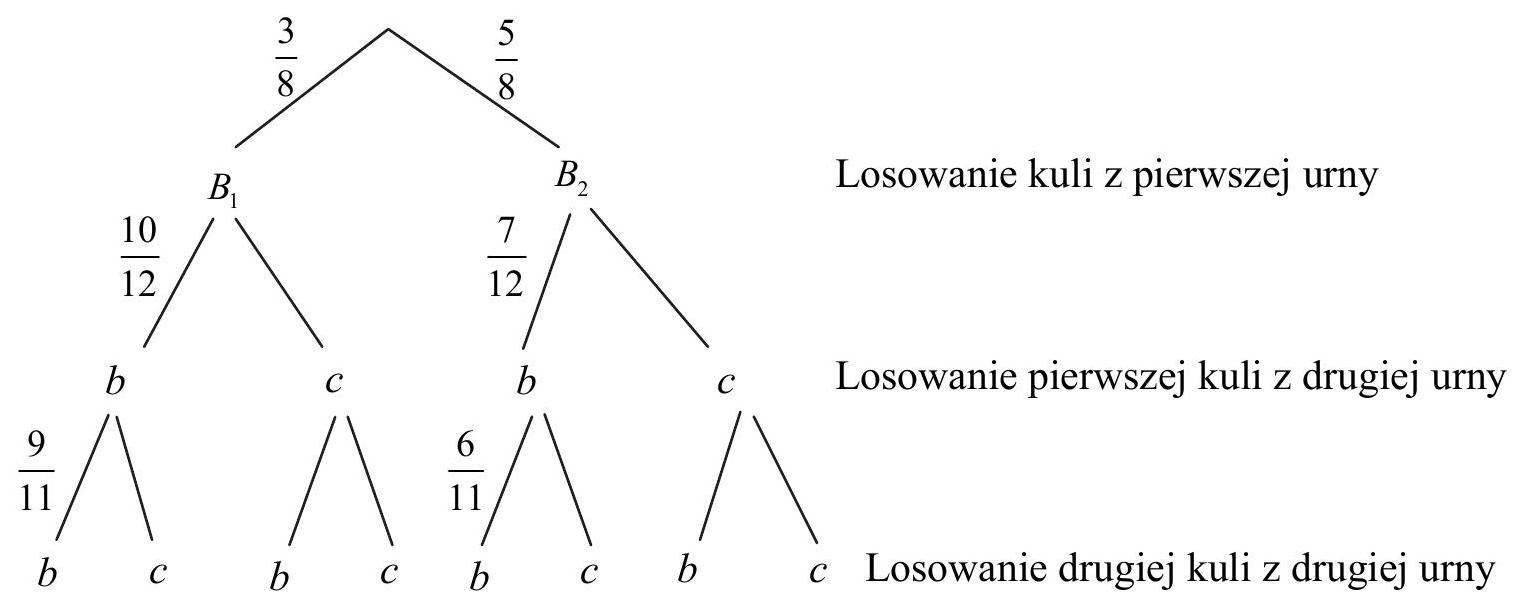
\includegraphics[max width=\textwidth, center]{2025_02_07_f5f4e8f37e6baab02e47g-16(1)}

Prawdopodobieństwo zdarzenia $A$ jest równe

$$
P(A)=\frac{15}{22} \cdot \frac{3}{8}+\frac{7}{22} \cdot \frac{5}{8}=\frac{45+35}{8 \cdot 22}=\frac{80}{8 \cdot 22}=\frac{5}{11}
$$

lub

$$
P(A)=\frac{\not{ }^{1}}{\not \mathscr{Q}^{4}} \cdot \frac{1 \sigma^{5}}{\not 2^{4}} \cdot \frac{9}{11}+\frac{5}{8} \cdot \frac{7}{\not \not 22} \cdot \frac{\not Q^{1}}{11}=\frac{45+35}{16 \cdot 11}=\frac{80}{176}=\frac{5}{11} .
$$

\section*{Schemat oceniania II sposobu rozwiązania}
Rozwiązanie, w którym postęp jest niewielki, ale konieczny na drodze do pełnego rozwiązania\\
Zdający narysuje drzewo ilustrujące losowanie (na rysunku muszą wystąpić wszystkie istotne gałęzie).\\
Rozwiązanie, w którym jest istotny postęp 2 p.\\
Zdający zapisze prawdopodobieństwa przynajmniej na wszystkich istotnych odcinkach jednego $z$ etapów lub na jednej $z$ istotnych gałęzi.

Pokonanie zasadniczych trudności zadania\\
Zdający zapisze prawdopodobieństwa na wszystkich istotnych gałęziach: $\frac{3}{8}, \frac{10}{12}, \frac{9}{11}$\\
oraz $\frac{5}{8}, \frac{7}{12}, \frac{6}{11}$ lub $\frac{3}{8}, \frac{\binom{10}{2}}{\binom{12}{2}}$ oraz $\frac{5}{8}, \frac{\binom{7}{2}}{\binom{12}{2}}$.\\
Rozwiązanie pelne 4 p.\\
Zdający obliczy prawdopodobieństwo: $P(A)=\frac{5}{11}$.

\section*{Uwaga}
Jeżeli zdający rozwiąże zadanie do końca i otrzyma prawdopodobieństwo ujemne lub większe od 1 , to za całe rozwiązanie otrzymuje 0 punktów.

Zadanie 12. (0-4)\\
Funkcja $f$ określona jest wzorem $f(x)=x^{3}-2 x^{2}+1$ dla każdej liczby rzeczywistej $x$. Wyznacz równania tych stycznych do wykresu funkcji $f$, które są równoległe do prostej o równaniu $y=4 x$.

\begin{center}
\begin{tabular}{|l|l|}
\hline
 & \begin{tabular}{l}
11. Rachunek różniczkowy. Zdający korzysta z geometrycznej \\
IV. Użycie i tworzenie \\
strategii. \\
\end{tabular} \\
\begin{tabular}{l}
i fizycznej interpretacji pochodnej (R11.3). \\
8. Geometria na płaszczyźnie kartezjańskiej. Zdający \\
wyznacza równania prostej, która jest równoległa lub \\
prostopadła do prostej danej w postaci kierunkowej \\
i przechodzi przez dany punkt (8.3). \\
\end{tabular} &  \\
\hline
\end{tabular}
\end{center}

\section*{Rozwiązanie}
Aby styczne były równoległe do prostej o równaniu $y=4 x$, ich współczynnik kierunkowy musi być równy 4 . Obliczamy pochodną funkcji $f: f^{\prime}(x)=3 x^{2}-4 x$.\\
Współczynnik kierunkowy stycznej jest równy wartości pierwszej pochodnej funkcji w punkcie styczności. Stąd $4=f^{\prime}\left(x_{0}\right)$. Wówczas

$$
\begin{gathered}
3 x_{0}^{2}-4 x_{0}=4, \\
3 x_{0}^{2}-4 x_{0}-4=0, \\
\Delta=64, \\
x_{0}=-\frac{2}{3} \text { lub } x_{0}=2 .
\end{gathered}
$$

Istnieją zatem dwie styczne do wykresu funkcji $f$ równoległe do prostej o równaniu $y=4 x$ w punktach $P_{1}=\left(-\frac{2}{3},-\frac{5}{27}\right)$ oraz $P_{2}=(2,1)$. Styczne mają zatem równania postaci

$$
y+\frac{5}{27}=4\left(x+\frac{2}{3}\right) \text { oraz } y-1=4(x-2), \text { czyli } y+=4 x+\frac{67}{27} \text { oraz } y=4 x-7
$$

Odp. Równania prostych stycznych mają postać: $y=4 x+\frac{67}{27}$ oraz $y=4 x-7$.

\section*{Schemat oceniania}
Rozwiązanie, w którym postęp jest niewielki, ale konieczny na drodze do pełnego\\
rozwiązania zadania................................................................................................... 1 p.\\
Zdający

\begin{itemize}
  \item obliczy pochodną funkcji $f: f^{\prime}(x)=3 x^{2}-4 x$\\
albo
  \item zapisze warunek $f^{\prime}\left(x_{0}\right)=4$.
\end{itemize}

Rozwiązanie, w którym jest istotny postęp\\
Zdający obliczy pochodną funkcji $f: f^{\prime}(x)=3 x^{2}-4 x$ i zapisze warunek $f^{\prime}\left(x_{0}\right)=4$.\\
Pokonanie zasadniczych trudności zadania.\\
Zdający rozwiąże równanie $3 x_{0}{ }^{2}-4 x_{0}=4$ i obliczy współrzędne obu punktów styczności:\\
$P_{1}=\left(-\frac{2}{3},-\frac{5}{27}\right), P_{2}=(2,1)$

\section*{Uwaga}
Jeżeli zdający korzysta ze wzoru $y=f^{\prime}\left(x_{0}\right) x+b$, gdzie $b=f\left(x_{0}\right)-f^{\prime}\left(x_{0}\right) \cdot x_{0}$, to obliczenie współczynnika $b$ traktujemy jak obliczenie drugiej współrzędnej punktu styczności.\\
Rozwiązanie pełne\\
Wyznaczenie równań stycznych: $y=4 x+\frac{67}{27}$ i $y=4 x-7$.

\section*{Uwaga}
Jeżeli zdający wyznaczy poprawnie współrzędne tylko jednego punktu styczności i w konsekwencji wyznaczy poprawnie równanie jednej stycznej, to otrzymuje $\mathbf{3}$ punkty.

\section*{Zadanie 13. (0-5)}
Dany jest trójmian kwadratowy $f(x)=(m+1) x^{2}+2(m-2) x-m+4$. Wyznacz wszystkie wartości parametru $m$, dla których trójmian $f$ ma dwa różne pierwiastki rzeczywiste $x_{1}, x_{2}$, spełniające warunek $x_{1}^{2}-x_{2}{ }^{2}=x_{1}^{4}-x_{2}{ }^{4}$.

\begin{center}
\begin{tabular}{|c|l}
\hline
\begin{tabular}{c}
III. Modelowanie \\
matematyczne. \\
\end{tabular} & \begin{tabular}{l}
3. Równania i nierówności. Zdający stosuje wzory Viète'a \\
(R3.1). \\
\end{tabular} \\
\hline
\end{tabular}
\end{center}

\section*{Rozwiązanie}
Z treści zadania wynika, że $m+1 \neq 0$, czyli $m \neq-1$.\\
Trójmian $f$ ma dwa różne pierwiastki rzeczywiste, gdy jego wyróżnik jest dodatni, czyli

$$
\begin{gathered}
\Delta=(2(m-2))^{2}-4 \cdot(m+1) \cdot(-m+4)>0, \\
8 m^{2}-28 m>0, \\
4 m(2 m-7)>0 .
\end{gathered}
$$

Stąd $m \in(-\infty, 0) \cup\left(\frac{7}{2},+\infty\right)$.\\
$D=(-\infty,-1) \cup(-1,0) \cup\left(\frac{7}{2},+\infty\right)$ jest zbiorem wszystkich wartości parametru $m$, dla których funkcja $f$ jest trójmianem kwadratowym i ma dwa różne pierwiastki.\\
Warunek $x_{1}^{2}-x_{2}^{2}=x_{1}^{4}-x_{2}^{4}$ możemy zapisać w postaci równoważnej

$$
\begin{gathered}
x_{1}^{2}-x_{2}^{2}=\left(x_{1}^{2}+x_{2}^{2}\right)\left(x_{1}^{2}-x_{2}^{2}\right), \\
\left.\left(x_{1}-x_{2}\right)\left(x_{1}+x_{2}\right)\left(1-\left(x_{1}^{2}+x_{2}^{2}\right)\right)\right)=0 .
\end{gathered}
$$

Stąd

$$
x_{1}-x_{2}=0 \text { lub } x_{1}+x_{2}=0 \text { lub } 1-\left(x_{1}^{2}+x_{2}^{2}\right)=0 .
$$

Równość $x_{1}-x_{2}=0$ przeczy założeniu $x_{1} \neq x_{2}$.\\
Ze wzoru Viète'a na sumę pierwiastków trójmianu kwadratowego możemy równanie $x_{1}+x_{2}=0$ zapisać w postaci $\frac{-2(m-2)}{m+1}=0$. Stąd $m=2 \notin D$.\\
Równanie $1-\left(x_{1}^{2}+x_{2}^{2}\right)=0$ możemy zapisać w postaci równoważnej

$$
\left(x_{1}+x_{2}\right)^{2}-2 x_{1} x_{2}=1
$$

Ze wzorów Viète'a otrzymujemy

$$
\begin{gathered}
\left(\frac{-2(m-2)}{m+1}\right)^{2}-2 \cdot \frac{-m+4}{m+1}=1, \\
\frac{4\left(m^{2}-4 m+4\right)}{(m+1)^{2}}+\frac{2 m-8}{m+1}-1=0, \\
4 m^{2}-16 m+16+(2 m-8)(m+1)-(m+1)^{2}=0, \\
5 m^{2}-24 m+7=0
\end{gathered}
$$

Rozwiązaniami tego równania są liczby

$$
m_{1}=\frac{12-\sqrt{109}}{5} \notin D \text { oraz } m_{2}=\frac{12+\sqrt{109}}{5} \in D
$$

Istnieje zatem jedna wartość parametru $m=\frac{12+\sqrt{109}}{5}$, dla której trójmian $f$ ma dwa różne pierwiastki rzeczywiste spełniające warunek $x_{1}^{2}-x_{2}^{2}=x_{1}^{4}-x_{2}^{4}$.

\section*{Schemat oceniania}
Rozwiązanie zadania składa się z trzech etapów.\\
Pierwszy z nich polega na rozwiązaniu nierówności $\Delta>0: m \in(-\infty, 0) \cup\left(\frac{7}{2},+\infty\right)$.\\
Za poprawne rozwiązanie tego etapu zdający otrzymuje 1 punkt.

\section*{Uwaga}
Jeżeli zdający zapisze $\Delta \geq 0$, to za tę część otrzymuje $\mathbf{0}$ punktów.\\
Drugi etap polega na rozwiązaniu równania $x_{1}^{2}-x_{2}^{2}=x_{1}^{4}-x_{2}^{4}$.\\
Za tę część rozwiązania zdający otrzymuje $\mathbf{3}$ punkty.\\
Podział punktów za drugi etap rozwiązania:\\
1 punkt zdający otrzymuje za zapisanie równania w postaci:

$$
\left(x_{1}-x_{2}\right)\left(x_{1}+x_{2}\right)\left(1-\left(x_{1}^{2}+x_{2}^{2}\right)\right)=0 \text { lub równoważnej. }
$$

2 punkty zdający otrzymuje za:

\begin{itemize}
  \item zapisanie równości $x_{1}-x_{2}=0$ i stwierdzenie, że przeczy ona założeniu $x_{1} \neq x_{2}$\\
albo
  \item rozwiązanie równania $\frac{-2(m-2)}{m+1}=0: m=2$\\
albo
  \item zapisanie równania $1-\left(x_{1}^{2}+x_{2}^{2}\right)=0$ w postaci, np.: $\left(\frac{-2(m-2)}{m+1}\right)^{2}-2 \cdot \frac{-m+4}{m+1}=1$.
\end{itemize}

3 punkty zdający otrzymuje za:

\begin{itemize}
  \item rozwiązanie równania $\frac{-2(m-2)}{m+1}=0: m=2$\\
oraz
  \item rozwiązanie równania $\left(\frac{-2(m-2)}{m+1}\right)^{2}-2 \cdot \frac{-m+4}{m+1}=1: m_{1}=\frac{12-\sqrt{109}}{5}$, $m_{2}=\frac{12+\sqrt{109}}{5}$.\\
Trzeci etap polega na wyznaczeniu szukanej wartości parametru $m$ : $m=\frac{12+\sqrt{109}}{5}$. Za ten etap zdający otrzymuje 1 punkt, o ile poprawnie wykona etapy I i II rozwiązania albo poprawnie wykona etap I i popełnia błędy w rozwiązaniu równania z etapu II, albo gdy popełnia błędy w etapie I i dobrze rozwiąże równanie z etapu II.
\end{itemize}

\section*{Uwagi:}
\begin{enumerate}
  \item Akceptujemy rozwiązania, w których zdający nie zapisuje założenia $m+1 \neq 0$, które wynika ze sformułowania zadania.
  \item Zdający nie musi rozwiązywać nierówności $\Delta>0$, o ile sprawdzi czy dla $m=2$, $m=\frac{12-\sqrt{109}}{5}, m=\frac{12+\sqrt{109}}{5}$ trójmian ma dwa różne pierwiastki rzeczywiste.
  \item Jeżeli zdający podzieli obie strony równania $x_{1}^{2}-x_{2}^{2}=x_{1}^{4}-x_{2}^{4}$ przez $x_{1}^{2}-x_{2}^{2}$ bez stosownego założenia i rozwiąże równanie $1=x_{1}^{2}+x_{2}^{2}$, otrzymując $m=\frac{12-\sqrt{109}}{5}$ lub $m=\frac{12+\sqrt{109}}{5}$, to otrzymuje co najwyżej 3 punkty za całe rozwiązanie, przy czym 1 punkt może otrzymać za rozwiązanie nierówności $\Delta>0$, $\mathbf{1}$ punkt za zapisanie równania $1=x_{1}^{2}+x_{2}^{2} \quad \mathrm{w}$ postaci równania wymiernego z jedną niewiadomą, np.: $\left(\frac{-2(m-2)}{m+1}\right)^{2}-2 \cdot \frac{-m+4}{m+1}=1$ oraz $\mathbf{1}$ punkt za wyznaczenie tego rozwiązania równania, które spełnia nierówność $\Delta>0$.
  \item Jeżeli zdający nie rozwiązywał nierówności $\Delta>0$, ale rozwiązał równanie $\left(\frac{-2(m-2)}{m+1}\right)^{2}-2 \cdot \frac{-m+4}{m+1}=1$ i sprawdził, dla której z otrzymanych wartości $m$ trójmian ma pierwiastki rzeczywiste, to otrzymuje $\mathbf{3}$ punkty.
\end{enumerate}

\section*{Zadanie 14. (0-5)}
Podstawą ostrosłupa $A B C D S$ jest kwadrat $A B C D$. Krawędź boczna $S D$ jest wysokością ostrosłupa, a jej długość jest dwa razy większa od długości krawędzi podstawy. Oblicz sinus kąta między ścianami bocznymi $A B S$ i $C B S$ tego ostrosłupa.

\section*{IV. Użycie i tworzenie}
 strategii.\begin{displayquote}

\begin{enumerate}
  \setcounter{enumi}{8}
  \item Stereometria. Zdający stosuje trygonometrię do obliczeń długości odcinków, miar kątów, pól powierzchni i objętości (9.6).
\end{enumerate}
\end{displayquote}

\section*{Rozwiązanie (I sposób)}
Przyjmijmy oznaczenia jak na rysunku.\\
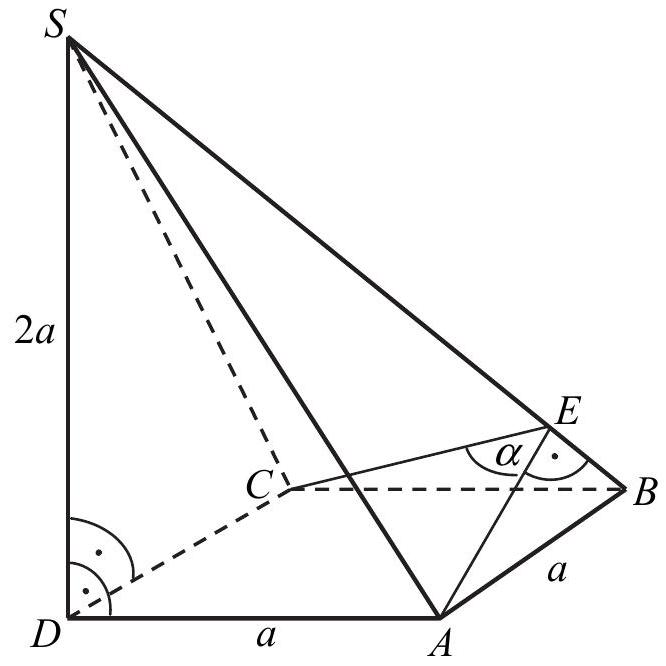
\includegraphics[max width=\textwidth, center]{2025_02_07_f5f4e8f37e6baab02e47g-22}

Długość przekątnej podstawy ostrosłupa jest równa $|A C|=a \sqrt{2}$.\\
Trójkąty $A D S$ i $C D S$ są przystające (oba są prostokątne, mają wspólną przyprostokątną $D S$ oraz $|A D|=|C D|$ ), więc krawędzie boczne $A S$ i $C S$ ostrosłupa mają tę samą długość.\\
Z twierdzenia Pitagorasa

$$
|S A|=|S C|=\sqrt{(2 a)^{2}+a^{2}}=a \sqrt{5} .
$$

Trójkąt $A B S$ jest prostokątny, więc z twierdzenia Pitagorasa

$$
|S B|=\sqrt{(a \sqrt{5})^{2}+a^{2}}=a \sqrt{6} .
$$

Odcinek $A E$ jest wysokością ściany bocznej $A B S$. Jego długość możemy wyznaczyć zapisując np. pole trójkąta $A B S$ na dwa sposoby

$$
\frac{1}{2} a \cdot a \sqrt{5}=\frac{1}{2} a \sqrt{6} \cdot|A E|, \text { stąd }|A E|=a \sqrt{\frac{5}{6}}=|C E| .
$$

Z twierdzenia cosinusów dla trójkąta $A E C$ otrzymujemy

$$
2 a^{2}=\frac{5}{6} a^{2}+\frac{5}{6} a^{2}-2 \cdot \frac{5}{6} a^{2} \cos \alpha .
$$

Stąd $\cos \alpha=-\frac{1}{5}$. Zatem $\sin \alpha=\frac{2 \sqrt{6}}{5}$.

\section*{Rozwiązanie (II sposób)}
Przyjmijmy oznaczenia jak na rysunku.\\
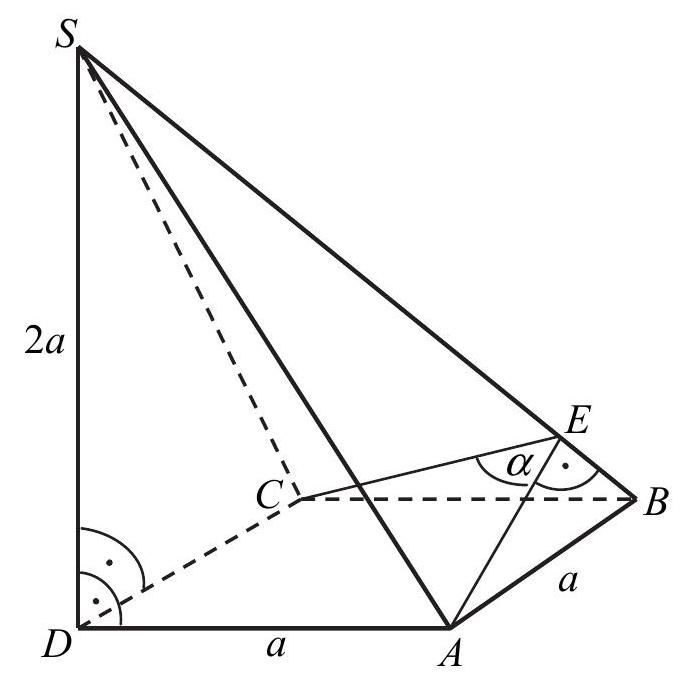
\includegraphics[max width=\textwidth, center]{2025_02_07_f5f4e8f37e6baab02e47g-23}

Długość przekątnej podstawy ostrosłupa jest równa $|A C|=|B D|=a \sqrt{2}$.\\
Trójkąty $A D S$ i $C D S$ są przystające (oba są prostokątne, mają wspólną przyprostokątną $D S$ oraz $|A D|=|C D|$ ), więc krawędzie boczne $A S$ i $C S$ ostrosłupa mają tę samą długość. Z twierdzenia Pitagorasa

$$
|S A|=|S C|=\sqrt{(2 a)^{2}+a^{2}}=a \sqrt{5}
$$

Trójkąt $B D S$ jest prostokątny, więc z twierdzenia Pitagorasa

$$
|S B|=\sqrt{(2 a)^{2}+(a \sqrt{2})^{2}}=a \sqrt{6} .
$$

Odcinek $A E$ jest wysokością ściany bocznej $A B S$. Jego długość możemy wyznaczyć zapisując np. pole trójkąta $A B S$ na dwa sposoby

$$
\frac{1}{2} a \cdot a \sqrt{5}=\frac{1}{2} a \sqrt{6} \cdot|A E|, \text { stąd }|A E|=a \sqrt{\frac{5}{6}}=|C E|
$$

Z twierdzenia cosinusów dla trójkąta $A E C$ otrzymujemy

$$
2 a^{2}=\frac{5}{6} a^{2}+\frac{5}{6} a^{2}-2 \cdot \frac{5}{6} a^{2} \cos \alpha
$$

Stąd $\cos \alpha=-\frac{1}{5}$. Zatem $\sin \alpha=\frac{2 \sqrt{6}}{5}$.

\section*{Rozwiązanie (III sposób)}
Przyjmijmy oznaczenia jak na rysunku.\\
Długość przekątnej podstawy ostrosłupa jest równa $|A C|=|B D|=a \sqrt{2}$.\\
Trójkąty $A D S$ i $C D S$ są przystające (oba są prostokątne, mają wspólną przyprostokątną $D S$ oraz $|A D|=|C D|$ ), więc krawędzie boczne $A S$ i $C S$ ostrosłupa mają tę samą długość.\\
Z twierdzenia Pitagorasa

$$
|S A|=|S C|=\sqrt{(2 a)^{2}+a^{2}}=a \sqrt{5} .
$$

Trójkąt $B D S$ jest prostokątny, więc z twierdzenia Pitagorasa

$$
|S B|=\sqrt{(2 a)^{2}+(a \sqrt{2})^{2}}=a \sqrt{6}
$$

\begin{center}
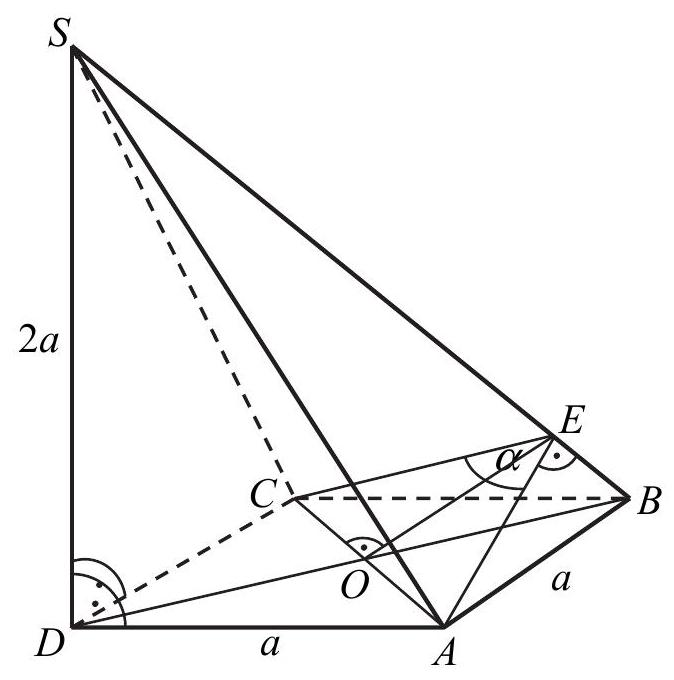
\includegraphics[max width=\textwidth]{2025_02_07_f5f4e8f37e6baab02e47g-24}
\end{center}

Odcinek $A E$ jest wysokością ściany bocznej $A B S$. Jego długość możemy wyznaczyć zapisując np. pole trójkąta $A B S$ na dwa sposoby

$$
\begin{gathered}
\frac{1}{2} a \cdot a \sqrt{5}=\frac{1}{2} a \sqrt{6} \cdot|A E|, \text { stąd }|A E|=a \sqrt{\frac{5}{6}}=|C E| \\
\sin \frac{\alpha}{2}=\frac{\frac{a \sqrt{2}}{2}}{a \sqrt{\frac{5}{6}}}=\sqrt{\frac{3}{5}}
\end{gathered}
$$

Zatem cosinus.

$$
\begin{gathered}
\cos \frac{\alpha}{2}=\sqrt{1-\sin ^{2} \frac{\alpha}{2}}=\sqrt{1-\frac{3}{5}}=\sqrt{\frac{2}{5}} . \\
\sin \alpha=2 \sin \frac{\alpha}{2} \cdot \cos \frac{\alpha}{2}=2 \cdot \sqrt{\frac{3}{5}} \cdot \sqrt{\frac{2}{5}}=\frac{2 \sqrt{6}}{5} .
\end{gathered}
$$

\section*{Rozwiązanie (IV sposób)}
Przyjmijmy oznaczenia jak na rysunku.\\
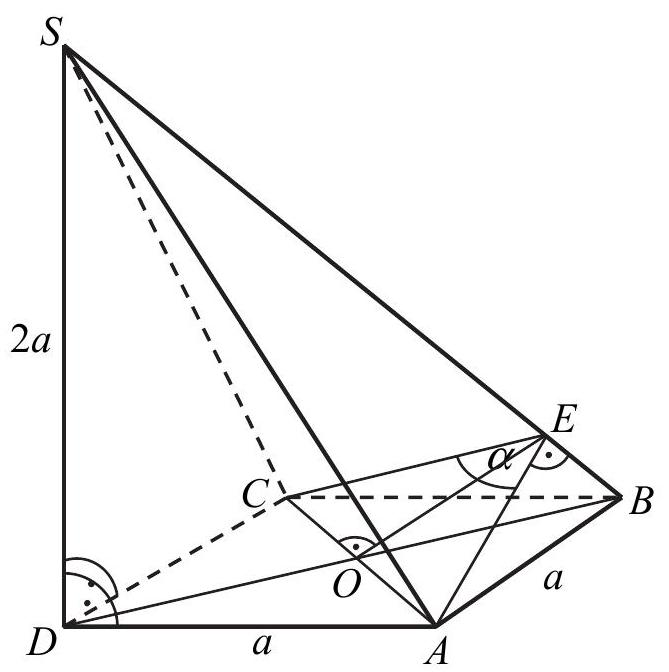
\includegraphics[max width=\textwidth, center]{2025_02_07_f5f4e8f37e6baab02e47g-24(1)}

Długość przekątnej podstawy ostrosłupa jest równa $|A C|=|B D|=a \sqrt{2}$.\\
Trójkąty $A D S$ i $C D S$ są przystające (oba są prostokątne, mają wspólną przyprostokątną $D S$ oraz $|A D|=|C D|$ ), więc krawędzie boczne $A S$ i $C S$ ostrosłupa mają tę samą długość.

Z twierdzenia Pitagorasa

$$
|S A|=|S C|=\sqrt{(2 a)^{2}+a^{2}}=a \sqrt{5} .
$$

Trójkąt $B D S$ jest prostokątny, więc z twierdzenia Pitagorasa

$$
|S B|=\sqrt{(2 a)^{2}+(a \sqrt{2})^{2}}=a \sqrt{6}
$$

Odcinek $A E$ jest wysokością ściany bocznej $A B S$. Jego długość możemy wyznaczyć zapisując np. pole trójkąta $A B S$ na dwa sposoby

$$
\frac{1}{2} a \cdot a \sqrt{5}=\frac{1}{2} a \sqrt{6} \cdot|A E|, \text { stąd }|A E|=a \sqrt{\frac{5}{6}}=|C E|
$$

Odcinek OE jest wysokością trójkąta $A E C$, więc $|O E|=a \frac{\sqrt{3}}{3}$.\\
Pole trójkąta $A E C$ możemy zapisać na dwa sposoby

$$
\frac{1}{2}|A E| \cdot|C E| \cdot \sin \alpha=\frac{1}{2}|A C| \cdot|O E|
$$

czyli

$$
\frac{1}{2} \cdot a \sqrt{\frac{5}{6}} \cdot a \sqrt{\frac{5}{6}} \cdot \sin \alpha=\frac{1}{2} \cdot a \sqrt{2} \cdot a \frac{\sqrt{3}}{3} .
$$

Stąd

$$
\sin \alpha=\frac{\sqrt{6}}{3} \cdot \frac{6}{5}=\frac{2 \sqrt{6}}{5} .
$$

\section*{Schemat oceniania}
Rozwiązanie, w którym postęp jest niewielki, ale konieczny na drodze do pełnego rozwiązania

\section*{Zdający}
\begin{itemize}
  \item wyznaczy długości krawędzi bocznych $S A, S C$ i $S B$ ostrosłupa $A B C D S$ :\\
$|S A|=|S C|=a \sqrt{5},|S B|=a \sqrt{6}$ i na tym poprzestanie lub dalej popełnienie błędów.
  \item zaznaczy poprawnie kąt między ścianami ABS i CBS.
\end{itemize}

Rozwiązanie, w którym jest istotny postęp\\
Zdający

\begin{itemize}
  \item wyznaczy długość odcinka $A E:|A E|=|C E|=a \sqrt{\frac{5}{6}}$\\
albo
  \item zapisze jedną z funkcji trygonometrycznych połowy kąta $\alpha:$ np. $\sin \frac{\alpha}{2}=\frac{|A O|}{|A E|}$.
\end{itemize}

Pokonanie zasadniczych trudności zadania 3 p.\\
Zdający

\begin{itemize}
  \item zapisze równanie wynikającego z twierdzenia cosinusów dla trójkąta $A E C$ :
\end{itemize}

$$
2 a^{2}=\frac{5}{6} a^{2}+\frac{5}{6} a^{2}-2 \cdot \frac{5}{6} a^{2} \cos \alpha
$$

albo

\begin{itemize}
  \item obliczy sinus połowy kąta $\alpha: \sin \frac{\alpha}{2}=\sqrt{\frac{3}{5}}$\\
albo
  \item obliczy wysokość $O E$ trójkąta $A C E:|O E|=\frac{a \sqrt{3}}{3}$.
\end{itemize}

\section*{Rozwiązanie prawie pełne}
4 p.\\
Zdający

\begin{itemize}
  \item obliczy cosinus kąta $A E C: \cos \alpha=-\frac{1}{5}$\\
albo
  \item zapisze równanie, z którego można obliczyć $\sin \alpha: \frac{1}{2} a \sqrt{\frac{5}{6}} \cdot a \sqrt{\frac{5}{6}} \sin \alpha=\frac{1}{2} a \sqrt{2} \cdot \frac{a \sqrt{3}}{3}$
\end{itemize}

\section*{Rozwiązanie pełne}
5 p.\\
Wyznaczenie sinusa kąta $A E C: \sin \alpha=\frac{2 \sqrt{6}}{5}$.

\section*{Uwaga}
Jeżeli zdający błędnie interpretuje kąt między ścianami bocznymi $A B S$ i $B C S$, to może otrzymać co najwyżej 1 punkt za wyznaczenie długości krawędzi bocznych.

Zadanie 15. (0-6)\\
Suma wszystkich czterech współczynników wielomianu $W(x)=x^{3}+a x^{2}+b x+c$ jest równa 0 . Trzy pierwiastki tego wielomianu tworzą ciąg arytmetyczny o różnicy równej 3. Oblicz współczynniki $a, b$ i $c$. Rozważ wszystkie możliwe przypadki.

\begin{center}
\begin{tabular}{|l|l|}
\hline
 & 5. Ciągi. Zdający stosuje wzór na $n$-ty wyraz i na sumę \\
IV. Użycie i tworzenie &  \\
strategii. & $n$ począkowych wyrazów ciągu arytmetycznego (5.3). \\
 & 13. Równania i nierówności. Zdający korzysta z własności \\
iloczynu przy rozwiązywaniu równań typu $x(x+1)(x-7)=0$ &  \\
 & $(3.7)$. \\
\end{tabular}
\end{center}

\section*{Rozwiązanie (I sposób)}
Suma współczynników wielomianu $W(x)=x^{3}+a x^{2}+b x+c$ jest równa $1+a+b+c=0$. Niech $p$ oznacza najmniejszy pierwiastek wielomianu $W$. Ponieważ pierwiastki wielomianu tworzą ciąg arytmetyczny o różnicy 3 , więc pozostałe dwa pierwiastki są równe $p+3$ oraz $p+6$.\\
a) Wielomian możemy więc zapisać w postaci iloczynowej

$$
W(x)=(x-p)(x-p-3)(x-p-6)
$$

Stąd

$$
\begin{gathered}
W(x)=\left(x^{2}-p x-3 x-p x+p^{2}+3 p\right)(x-p-6) \\
W(x)=x^{3}-p x^{2}-6 x^{2}-p x^{2}+p^{2} x+6 p x+p^{2} x-p^{3}-6 p^{2}+3 p x-3 p^{2}-18 p, \\
W(x)=x^{3}+(-3 p-9) x^{2}+\left(3 p^{2}+18 p+18\right) x+\left(-p^{3}-9 p^{2}-18 p\right)
\end{gathered}
$$

Porównujemy współczynniki wielomianu, otrzymując układ równań:

$$
\left\{\begin{array}{l}
a=-3 p-9 \\
b=3 p^{2}+18 p+18 \\
c=-p^{3}-9 p^{2}-18 p
\end{array}\right.
$$

b) Możemy zapisać układ równań

$$
\left\{\begin{array}{l}
p^{3}+a p^{2}+b p+c=0 \\
(p+3)^{3}+a(p+3)^{2}+b(p+3)+c=0 \\
(p+6)^{3}+a(p+6)^{2}+b(p+6)+c=0
\end{array}\right.
$$

Stąd po przekształceniach, otrzymujemy układ równań:

$$
\left\{\begin{array}{l}
a=-3 p-9 \\
b=3 p^{2}+18 p+18 \\
c=-p^{3}-9 p^{2}-18 p
\end{array}\right.
$$

c) Korzystając ze wzorów Viète’a $\left\{\begin{array}{l}x_{1}+x_{2}+x_{3}=-a \\ x_{1} \cdot x_{2}+x_{1} \cdot x_{3}+x_{2} \cdot x_{3}=b \\ x_{1} \cdot x_{2} \cdot x_{3}=-c\end{array}\right.$, możemy zapisać układ równań, otrzymując kolejno

$$
\left\{\begin{array}{l}
\left\{\begin{array}{l}
p+p+3+p+6=-a \\
p \cdot(p+3)+p \cdot(p+6)+(p+3) \cdot(p+6)=b \\
p \cdot(p+3) \cdot(p+6)=-c
\end{array}\right. \\
\left\{\begin{array}{l}
a=-3 p-9 \\
b=3 p^{2}+18 p+18 \\
c=-p^{3}-9 p^{2}-18 p
\end{array}\right.
\end{array}\right.
$$

Stąd i z równości $1+a+b+c=0$, otrzymujemy

$$
\begin{gathered}
(-3 p-9)+\left(3 p^{2}+18 p+18\right)+\left(-p^{3}-9 p^{2}-18 p\right)+1=0, \\
p^{3}+6 p^{2}+3 p-10=0 .
\end{gathered}
$$

Liczba 1 jest pierwiastkiem tego równania, więc z twierdzenia Bézouta wynika, że wielomian $p^{3}+6 p^{2}+3 p-10$ jest podzielny przez dwumian $p-1$.\\
Wykonujemy dzielenie, stosując np. schemat Hornera.

\begin{center}
\begin{tabular}{|c|c|c|c|c|}
\hline
 & 1 & 6 & 3 & -10 \\
\hline
1 & 1 & 7 & 10 & 0 \\
\hline
\end{tabular}
\end{center}

Równanie możemy więc zapisać w postaci $(p-1)\left(p^{2}+7 p+10\right)=0$.\\
Pozostałe rozwiązania równania $p^{3}+6 p^{2}+3 p-10=0$ to pierwiastki trójmianu kwadratowego $p^{2}+7 p+10$, czyli liczby $p=-5, p=-2$.\\
Gdy $p=1$, to wtedy $a=-12, b=39, c=-28$.\\
Gdy $p=-5$, to wtedy $a=6, b=3, c=-10$.\\
Gdy $p=-2$, to wtedy $a=-3, b=-6, c=8$.\\
Odpowiedź: Współczynniki $a, b, c$ są równe: $\left\{\begin{array}{l}a=-12 \\ b=39 \\ c=-28\end{array}\right.$ lub $\left\{\begin{array}{l}a=-3 \\ b=-6 \\ c=8\end{array}\right.$ lub $\left\{\begin{array}{l}a=6 \\ b=3 \\ c=-10\end{array}\right.$

\section*{Rozwiązanie (II sposób)}
Z równości $1+a+b+c=0$ otrzymujemy $c=-1-a-b$. Wielomian $W$ możemy zapisać w postaci

$$
\begin{gathered}
W(x)=x^{3}+a x^{2}+b x-1-a-b, \\
W(x)=x^{3}-1+a x^{2}-a+b x-b, \\
W(x)=(x-1)\left(x^{2}+x+1\right)+a\left(x^{2}-1\right)+b(x-1), \\
W(x)=(x-1)\left(x^{2}+(a+1) x+a+b+1\right) .
\end{gathered}
$$

Stąd wynika, że liczba $x=1$ jest pierwiastkiem wielomianu $W$.\\
Dalszą część rozwiązania możemy przeprowadzić na dwa sposoby\\
a) Pierwiastki tego wielomianu tworzą ciąg arytmetyczny o różnicy równej 3 , więc mamy trzy takie ciągi $(1,4,7),(-2,1,4),(-5,-2,1)$. Wielomian możemy wówczas zapisać\\
w postaci iloczynowej, odpowiednio:\\
$W(x)=(x-1)(x-4)(x-7), W(x)=(x+2)(x-1)(x-4), W(x)=(x+5)(x+2)(x-1)$.\\
Po doprowadzeniu do postaci uporządkowanej mamy $W(x)=x^{3}-12 x^{2}+39 x-28, W(x)=x^{3}-3 x^{2}-6 x+8, W(x)=x^{3}+6 x^{2}+3 x-10$.\\
Wyznaczamy odpowiednio współczynniki wielomianu $W$ :\\
$(a=-12, b=39, c=-28)$ lub $(a=-3, b=-6, c=8)$ lub $(a=6, b=3, c=-10)$.\\
b) Niech $x_{1}$ i $x_{2}$ oznaczają pierwiastki trójmianu $T(x)=x^{2}+(a+1) x+a+b+1$. Możemy założyć, że $x_{1} \leq x_{2}$. Pierwiastki wielomianu $W$ tworzą ciąg arytmetyczny, więc z własności ciągu arytmetycznego otrzymujemy np.:

$$
\left(x_{1}=4, x_{2}=7\right) \operatorname{lub}\left(x_{1}=-2, x_{2}=4\right) \operatorname{lub}\left(x_{1}=-5, x_{2}=-2\right)
$$

Korzystając ze wzorów Viète'a, otrzymujemy trzy układy równań

$$
\begin{gathered}
\left\{\begin{array} { l } 
{ 4 + 7 = - ( a + 1 ) } \\
{ 4 \cdot 7 = a + b + 1 }
\end{array} \text { lub } \left\{\begin{array}{l}
-2+4=-(a+1) \\
-2 \cdot 4=a+b+1
\end{array}\right.\right. \text { lub }
\end{gathered}\left\{\begin{array}{l}
-5-2=-(a+1) \\
-5 \cdot(-2)=a+b+1
\end{array}\right\}
$$

Obliczamy odpowiednio $c=-1-a-b$ :

$$
\left\{\begin{array} { l } 
{ a = - 1 2 } \\
{ b = 3 9 } \\
{ c = - 2 8 }
\end{array} \text { lub } \left\{\begin{array} { l } 
{ a = - 3 } \\
{ b = - 6 } \\
{ c = 8 }
\end{array} \quad \text { lub } \quad \left\{\begin{array}{l}
a=6 \\
b=3 \\
c=-10
\end{array}\right.\right.\right.
$$

\section*{Rozwiązanie (III sposób)}
Suma współczynników wielomianu $W(x)=x^{3}+a x^{2}+b x+c$ jest równa $1+a+b+c=0$. Z równości $1+a+b+c=0$ wynika, że liczba 1 jest pierwiastkiem wielomianu $W$.\\
Ponieważ pierwiastki wielomianu tworzą ciąg arytmetyczny o różnicy 3 , to możemy zapisać trzy ciągi arytmetyczne, których jednym z wyrazów jest liczba $1:(1,4,7),(-2,1,4)$, $(-5,-2,1)$.

Stąd wielomian $W$ możemy więc zapisać w postaci:\\
$W(x)=(x-1)(x-4)(x-7)$ lub $W(x)=(x+2)(x-1)(x-4)$,\\
lub $W(x)=(x+5)(x+2)(x-1)$\\
Po doprowadzeniu do postaci uporządkowanej mamy

$$
W(x)=x^{3}-12 x^{2}+39 x-28 \text { lub } W(x)=x^{3}-3 x^{2}-6 x+8, \text { lub } W(x)=x^{3}+6 x^{2}+3 x-10 .
$$

Wyznaczamy współczynniki wielomianu $W$ :

$$
(a=-12, b=39, c=-28) \operatorname{lub}(a=-3, b=-6, c=8), \operatorname{lub}(a=6, b=3, c=-10) .
$$

\section*{Schemat oceniania}
Rozwiązanie, w którym postęp jest niewielki, ale konieczny na drodze do pełnego rozwiązania 1 p.\\
Zdający

\begin{itemize}
  \item zapisze wielomian $W$ w postaci iloczynowej, np .: $W(x)=(x-p)(x-p-3)(x-p-6)$, gdzie $p$ jest pierwiastkiem wielomianu\\
albo
  \item zapisze układ równań, gdzie $p$ jest pierwiastkiem wielomianu
\end{itemize}

$$
\left\{\begin{array}{l}
p^{3}+a p^{2}+b p+c=0 \\
(p+3)^{3}+a(p+3)^{2}+b(p+3)+c=0 \\
(p+6)^{3}+a(p+6)^{2}+b(p+6)+c=0
\end{array}\right.
$$

albo

\begin{itemize}
  \item zapisze układ równań, korzystając ze wzorów Viète’a
\end{itemize}

$$
\left\{\begin{array}{l}
p+p+3+p+6=-a \\
p \cdot(p+3)+p \cdot(p+6)+(p+3) \cdot(p+6)=b \\
p \cdot(p+3) \cdot(p+6)=-c
\end{array}\right.
$$

albo

\begin{itemize}
  \item wyznaczy $c=-1-a-b$ i zapisze wielomian $W \mathrm{w}$ postaci
\end{itemize}

$$
W(x)=x^{3}-1+a\left(x^{2}-1\right)+b(x-1)
$$

Rozwiązanie, w którym jest istotny postęp.\\
2 p.\\
Zdający zapisze

\begin{itemize}
  \item układ równań: $\left\{\begin{array}{l}a=-3 p-9 \\ b=3 p^{2}+18 p+18 \\ c=-p^{3}-9 p^{2}-18 p\end{array}\right.$\\
albo
  \item wielomian $W$ w postaci iloczynu: $W(x)=(x-1)\left(x^{2}+(a+1) x+a+b+1\right)$\\
albo
  \item zapisze, że z równości $1+a+b+c=0$ wynika, że liczba 1 jest pierwiastkiem wielomianu $W$\\
albo
  \item zapisze układ czterech równań z 4 niewiadomymi, np.\\
$\left\{\begin{array}{l}p+p+3+p+6=-a \\ p \cdot(p+3)+p \cdot(p+6)+(p+3) \cdot(p+6)=b \\ p \cdot(p+3) \cdot(p+6)=-c \\ 1+a+b+c=0\end{array}\right.$
\end{itemize}

\section*{Zdający}
\begin{itemize}
  \item wyznaczy wszystkie rozwiązania równania $p^{3}+6 p^{2}+3 p-10=0: 1,-2,-5$\\
albo
  \item zauważy, że liczba 1 jest pierwiastkiem wielomianu $W$ i zapisze trzy ciągi arytmetyczne o różnicy 3 , których jednym z wyrazów jest liczba 1 :\\
$(1,4,7),(-2,1,4),(-5,-2,1)$\\
albo
  \item zauważy, że liczba 1 jest pierwiastkiem wielomianu $W$ i zapisze jeden ciąg arytmetyczny o różnicy 3 , w którym jednym z wyrazów jest liczba 1 : np. $(1,4,7)$ lub $(-2,1,4)$, lub $(-5,-2,1)$ i dla tego ciągu obliczy współczynniki $a, b, c$ wielomianu, to otrzymuje $\mathbf{4}$ punkty.
\end{itemize}

\section*{Uwagi:}
\begin{itemize}
  \item Jeżeli zdający wyznaczy jeden z pierwiastków wielomianu $W$ i wykorzystuje informację, że pierwiastki wielomianu są kolejnymi wyrazami ciągu arytmetycznego, to otrzymuje $\mathbf{3}$ punkty.
  \item Jeżeli zdający zapisze równanie z jedną niewiadomą, np. $p^{3}+6 p^{2}+3 p-10=0$, to otrzymuje 3 punkty.
\end{itemize}

\section*{Rozwiązanie zadania do końca, lecz z usterkami, które jednak nie przekreślają lub poprawności rozwiązania (np. błędy rachunkowe) 5 p.}
Zdający

\begin{itemize}
  \item rozwiąże zadanie do końca, popełniając błędy rachunkowe\\
albo
  \item zapisze, że z równości $1+a+b+c=0$ wynika, że liczba 1 jest pierwiastkiem wielomianu $W$, zapisze trzy ciągi arytmetyczne o różnicy 3, których jednym z wyrazów jest liczba 1: $(1,4,7),(-2,1,4),(-5,-2,1)$ oraz zapisze, że $W(x)=(x-1)(x-4)(x-7)$ lub $W(x)=(x+2)(x-1)(x-4)$, lub $W(x)=(x+5)(x+2)(x-1)$.\\
albo
  \item wyznaczy współczynniki $a, b, c$ wielomianu tylko dla dwóch ciągów
\end{itemize}

Rozwiązanie petne 6 p.\\
Zdający wyznaczy współczynniki wielomianu $W$ : $(a=-12, b=39, c=-28)$ lub $(a=-3$, $b=-6, c=8)$, lub ( $a=6, b=3, c=-10)$.

\section*{Zadanie 16. (0-7)}
Rozpatrujemy wszystkie stożki, których przekrojem osiowym jest trójkąt o obwodzie 20. Oblicz wysokość i promień podstawy tego stożka, którego objętość jest największa. Oblicz objętość tego stożka.

\begin{center}
\begin{tabular}{|c|l|}
\hline
\begin{tabular}{c}
III. Modelowanie \\
matematyczne. \\
\end{tabular} & \begin{tabular}{l}
11. Rachunek różniczkowy. Zdający stosuje pochodne do \\
rozwiązywania zagadnień optymalizacyjnych (R11.6). \\
\end{tabular} \\
\hline
\end{tabular}
\end{center}

\section*{Rozwiązanie (I sposób)}
Przyjmijmy oznaczenia jak na rysunku.\\
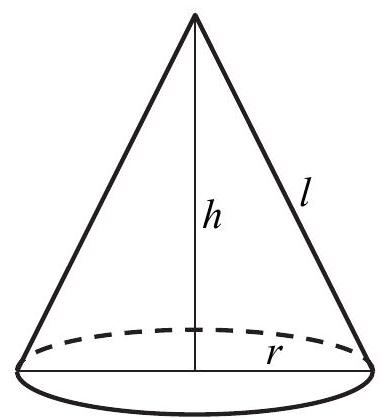
\includegraphics[max width=\textwidth, center]{2025_02_07_f5f4e8f37e6baab02e47g-32}

Objętość stożka wyraża się wzorem

$$
V=\frac{1}{3} \cdot \pi r^{2} h .
$$

Przekrój osiowy stożka jest trójkątem równoramiennym, którego obwód jest równy 20, więc

$$
\begin{gathered}
2 r+2 l=20 \\
r+l=10 \\
l=10-r
\end{gathered}
$$

Stąd i z twierdzenia Pitagorasa otrzymujemy

$$
\begin{gathered}
r^{2}+h^{2}=l^{2}, \\
r^{2}=l^{2}-h^{2}, \\
r^{2}=(10-r)^{2}-h^{2}, \\
h^{2}=100-20 r .
\end{gathered}
$$

Zatem $h=\sqrt{100-20 r}$.\\
Z geometrycznych warunków zadania otrzymujemy $0<r<5$.\\
Zapisujemy objętość stożka w zależności od zmiennej $r$

$$
V(r)=\frac{1}{3} \cdot \pi r^{2} \cdot \sqrt{100-20 r}
$$

Wzór tej funkcji zapiszemy w postaci $V(r)=\frac{1}{3} \cdot \pi \sqrt{100 r^{4}-20 r^{5}}$ dla $0<r<5$.\\
Rozważmy funkcję pomocniczą określoną wzorem $f(r)=100 r^{4}-20 r^{5}$ dla $0<r<5$.

Z faktu, że funkcja $g(t)=\sqrt{t}$ jest rosnąca $\mathrm{w}\langle 0,+\infty)$ wynika, że funkcje $V$ oraz $f$ są rosnące (malejące) w tych samych przedziałach oraz mają ekstrema lokalne (tego samego rodzaju) dla tych samych argumentów.\\
Wyznaczamy wartość największą funkcji $f \mathrm{w}$ przedziale $(0,5)$.\\
Obliczamy pochodną funkcji $f$ :

$$
f^{\prime}(r)=400 r^{3}-100 r^{4}
$$

W przedziale $(0,5)$ pochodna ma jedno miejsce zerowe $r=4$. Ponadto

$$
\begin{aligned}
& f^{\prime}(r)>0 \text { dla } r \in(0,4), \\
& f^{\prime}(r)<0 \text { dla } r \in(4,5)
\end{aligned}
$$

Wynika stąd, że dla $x=4$ funkcja $f$ ma maksimum lokalne, które jest jednocześnie największą wartością funkcji $V$, bo w przedziale $(0,4\rangle$ funkcja $f$ jest rosnąca, a przedziale $\langle 4,0)$ funkcja $f$ jest malejąca.\\
Gdy $r=4$, to $h=\sqrt{100-20 \cdot 4}=\sqrt{20}=2 \sqrt{5}$, natomiast objętość stożka jest wówczas równa:

$$
V(4)=\frac{1}{3} \cdot \pi \cdot 4^{2} \cdot \sqrt{100-20 \cdot 4}=\frac{32 \pi \sqrt{5}}{3}
$$

Odp.: Największą objętość równą $\frac{32 \pi \sqrt{5}}{3}$ ma stożek o promieniu podstawy 4 i wysokości $2 \sqrt{5}$.

\section*{Schemat oceniania I sposobu rozwiązania}
Rozwiązanie zadania składa się z trzech etapów.\\
Pierwszy etap składa się z trzech części:

\begin{itemize}
  \item oznaczenia promienia podstawy stożka, np. $r$ i wyznaczenia wysokości stożka w zależności od zmiennej $r$ : $h=\sqrt{100-20 r}$.
  \item zapisania objętości $V$ stożka jako funkcji jednej zmiennej $V(r)=\frac{1}{3} \cdot \pi r^{2} \cdot \sqrt{100-20 r}$,
  \item zapisania dziedziny funkcji $V(r)=\frac{1}{3} \cdot \pi r^{2} \cdot \sqrt{100-20 r}: 0<r<5$.
\end{itemize}

Za drugą część tego etapu zdający może otrzymać punkt, o ile pierwszą cześć wykona bezbłędnie. Punkt za cześś trzecią otrzymuje niezależnie od realizacji dwóch pierwszy części tego etapu.

Drugi etap składa się z trzech części:

\begin{itemize}
  \item wyznaczenia wzoru pochodnej funkcji $f(r)=100 r^{4}-20 r^{5}: f^{\prime}(r)=400 r^{3}-100 r^{4}$,
  \item obliczenia miejsc zerowych pochodnej: $r_{1}=0, r_{2}=4$,
  \item zbadania znaku pochodnej funkcji $f: f^{\prime}(r)>0$ dla $r \in(0,4), f^{\prime}(r)<0$ dla $r \in(4,5)$ i zapisania, że dla $r=4$ funkcja $V$ osiąga największą wartość.
\end{itemize}

\section*{Uwagi:}
\begin{enumerate}
  \item Znak pochodnej zdający może zaznaczyć w inny sposób, np. na rysunku szkicując krzywą zbliżoną do wykresu pochodnej.
  \item Jeśli zdający nie wyznaczy dziedziny funkcji $V$ lub określi funkcję $f$ na zbiorze szerszym od dziedziny funkcji $V$, to punkt za tę cześć może otrzymać jedynie wtedy, gdy wskazuje jako największą wartość funkcji tylko to maksimum, które funkcja $f$ osiąga dla argumentu z dziedziny funkcji $V$.
\end{enumerate}

Za poprawne rozwiązanie każdej z części tego etapu zdający otrzymuje 1 punkt, o ile poprzednia część etapu została zrealizowana bezbłędnie.

\section*{Trzeci etap}
Zapisanie, że promień stożka o największej objętości jest równy $r=4$, wysokość $h=\sqrt{20}=2 \sqrt{5}$ i obliczenie największej objętości stożka $V(4)=\frac{32 \pi \sqrt{5}}{3}$. Za realizację tego etapu zdający otrzymuje $\mathbf{1}$ punkt.

\section*{Rozwiązanie (II sposób)}
Przyjmijmy oznaczenia jak na rysunku.\\
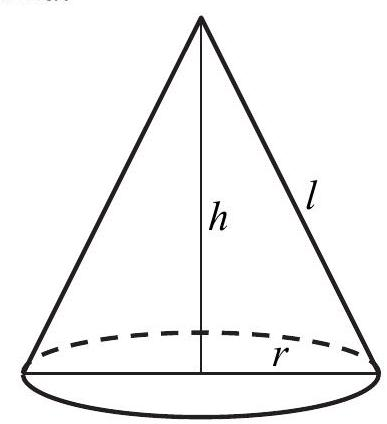
\includegraphics[max width=\textwidth, center]{2025_02_07_f5f4e8f37e6baab02e47g-34}

Objętość stożka wyraża się wzorem

$$
V=\frac{1}{3} \cdot \pi r^{2} h .
$$

Przekrój osiowy stożka jest trójkątem równoramiennym, którego obwód jest równy 20, więc

$$
\begin{gathered}
2 r+2 l=20 \\
r+l=10 \\
l=10-r
\end{gathered}
$$

Stąd i z twierdzenia Pitagorasa otrzymujemy

$$
\begin{gathered}
r^{2}+h^{2}=l^{2}, \\
r^{2}=l^{2}-h^{2}, \\
r^{2}=(10-r)^{2}-h^{2}, \\
h^{2}=100-20 r .
\end{gathered}
$$

Zatem $r=\frac{100-h^{2}}{20}=5-\frac{1}{20} h^{2}$.\\
Z geometrycznych warunków zadania otrzymujemy $0<h<10$. Zapisujemy objętość stożka w zależności od zmiennej $h$

$$
\begin{gathered}
V(h)=\frac{1}{3} \cdot \pi\left(5-\frac{1}{20} h^{2}\right)^{2} h, \\
V(h)=\frac{1}{3} \cdot \pi\left(25-\frac{1}{2} h^{2}+\frac{1}{400} h^{4}\right) \cdot h=\frac{\pi}{3} \cdot\left(25 h-\frac{1}{2} h^{3}+\frac{1}{400} h^{5}\right) \text { dla } 0<h<10 .
\end{gathered}
$$

Zauważamy, że wystarczy zbadać funkcję $f(h)=25 h-\frac{1}{2} h^{3}+\frac{1}{400} h^{5}$ określoną w przedziale $(0,10)$. Funkcje $V$ oraz $f$ są rosnące (malejące) w tych samych przedziałach oraz mają ekstrema lokalne (tego samego rodzaju) dla tych samych argumentów.\\
Wyznaczamy pochodną funkcji $f$ :

$$
f^{\prime}(h)=25-\frac{3}{2} h^{2}+\frac{1}{80} h^{4} .
$$

Następnie obliczamy miejsca zerowe pochodnej:

$$
\begin{gathered}
25-\frac{3}{2} h^{2}+\frac{1}{80} h^{4}=0 \text { i } t=h^{2} \\
\frac{1}{80} t^{2}-\frac{3}{2} t+25=0 \\
\Delta=\left(-\frac{3}{2}\right)^{2}-4 \cdot \frac{1}{80} \cdot 25=\frac{9}{4}-\frac{5}{4}=1 \\
t_{1}=\frac{\frac{3}{2}-1}{2 \cdot \frac{1}{80}}=20, \quad t_{2}=\frac{\frac{3}{2}+1}{2 \cdot \frac{1}{80}}=100 \\
h^{2}=20 \text { lub } h^{2}=100, \\
h=-2 \sqrt{5}, h=2 \sqrt{5}, h=-10, h=10 .
\end{gathered}
$$

Jedynym miejscem zerowym pochodnej funkcji $f$, które należy do przedziału $(0,10)$ jest

$$
h=2 \sqrt{5} .
$$

Ponadto:

$$
\begin{aligned}
& f^{\prime}(h)>0 \text { gdy } h \in(0,2 \sqrt{5}) \\
& f^{\prime}(h)<0 \text { gdy } h \in(2 \sqrt{5}, 10) .
\end{aligned}
$$

Stąd wynika, że dla $h=2 \sqrt{5}$ funkcja $f$ osiąga maksimum lokalne i jest to jednocześnie wartość największa, bo w przedziale $(0,2 \sqrt{5}\rangle$ funkcja $f$ jest rosnąca, a przedziale $\langle 2 \sqrt{5}, 10)$ funkcja $f$ jest malejąca.\\
Gdy $h=2 \sqrt{5}$, to $r=5-\frac{1}{20}(2 \sqrt{5})^{2}=4$ i objętość stożka jest wówczas równa:

$$
V(2 \sqrt{5})=\frac{1}{3} \cdot \pi \cdot 4^{2} \cdot 2 \sqrt{5}=\frac{32 \pi \sqrt{5}}{3}
$$

Odp.: Największą objętość równą $\frac{32 \pi \sqrt{5}}{3}$ ma stożek, którego promień jest równy 4 , a wysokośćc $2 \sqrt{5}$.

\section*{Schemat oceniania II sposobu rozwiązania}
Rozwiązanie zadania składa się z trzech etapów.\\
Pierwszy etap składa się z trzech czę̨ści:

\begin{itemize}
  \item oznaczenia wysokości stożka, np. $h$ i wyznaczenia promienia podstawy stożka w zależności od zmiennej $h: r=\frac{100-h^{2}}{20}=5-\frac{1}{20} h^{2}$,
  \item zapisania objętości $V$ stożka jako funkcji jednej zmiennej
\end{itemize}

$$
V(h)=\frac{1}{3} \cdot \pi\left(25-\frac{1}{2} h^{2}+\frac{1}{400} h^{4}\right) \cdot h=\frac{\pi}{3} \cdot\left(25 h-\frac{1}{2} h^{3}+\frac{1}{400} h^{5}\right),
$$

\begin{itemize}
  \item zapisania dziedziny funkcji $V(h)=\frac{\pi}{3} \cdot\left(25 h-\frac{1}{2} h^{3}+\frac{1}{400} h^{5}\right): 0<h<10$.
\end{itemize}

Za drugą część tego etapu zdający może otrzymać punkt, o ile pierwszą część wykona bezbłędnie. Punkt za część trzecią otrzymuje niezależnie od realizacji dwóch pierwszy części tego etapu.

Drugi etap składa się z trzech części:

\begin{itemize}
  \item wyznaczenia wzoru pochodnej funkcji $f(h)=25 h-\frac{1}{2} h^{3}+\frac{1}{400} h^{5}$ :
\end{itemize}

$$
f^{\prime}(h)=25-\frac{3}{2} h^{2}+\frac{1}{80} h^{4},
$$

\begin{itemize}
  \item obliczenia miejsc zerowych pochodnej: $h=-2 \sqrt{5}, h=2 \sqrt{5}, h=-10, h=10$,
  \item zbadania znaku pochodnej funkcji $f: f^{\prime}(h)>0$ dla $h \in(0,2 \sqrt{5}), f^{\prime}(h)<0$ dla\\
$h \in(2 \sqrt{5}, 10)$ i zapisania, że dla $h=2 \sqrt{5}$ funkcja $V$ osiąga największą wartość.
\end{itemize}

\section*{Uwagi:}
\begin{enumerate}
  \item Znak pochodnej zdający może zaznaczyć w inny sposób, np. na rysunku szkicując krzywą zbliżoną do wykresu pochodnej.
  \item Jeśli zdający nie wyznaczy dziedziny funkcji $V$ lub określi funkcję $f$ na zbiorze szerszym od dziedziny funkcji $V$, to punkt za tę cześć może otrzymać jedynie wtedy, gdy wskazuje jako największą wartość funkcji tylko to maksimum, które funkcja $f$ osiąga dla argumentu z dziedziny funkcji $V$, przy czym konieczne jest uzasadnienie, że jest to największa wartość funkcji $V$ lub że funkcja $V$ nie przyjmuje wartości dla liczb większych od 10 .
\end{enumerate}

Za poprawne rozwiązanie każdej z części tego etapu zdający otrzymuje 1 punkt, o ile poprzednia część etapu została zrealizowana bezbłędnie.

\section*{Trzeci etap}
Zapisanie, że promień stożka o największej objętości jest równy $r=4$, wysokość\\
$h=\sqrt{20}=2 \sqrt{5}$ i obliczenie największej objętości stożka $V(4)=\frac{32 \pi \sqrt{5}}{3}$. Za realizację tego etapu zdający otrzymuje 1 punkt.


\end{document}